\section{The NEW detector}
\label{sec.new}


\begin{figure}[hpt!]
\centering
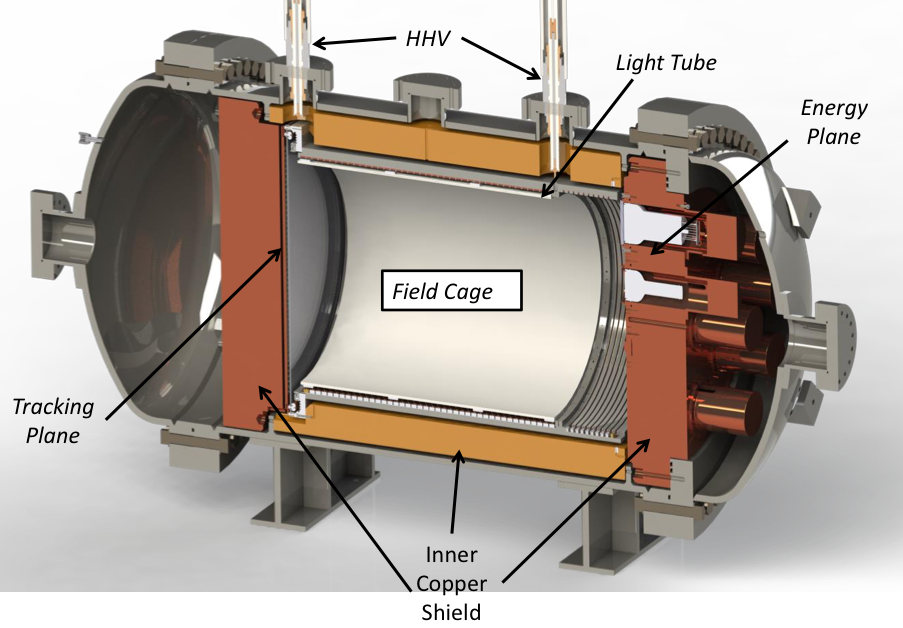
\includegraphics[height=8cm]{img2/NEWMay20163D.png}
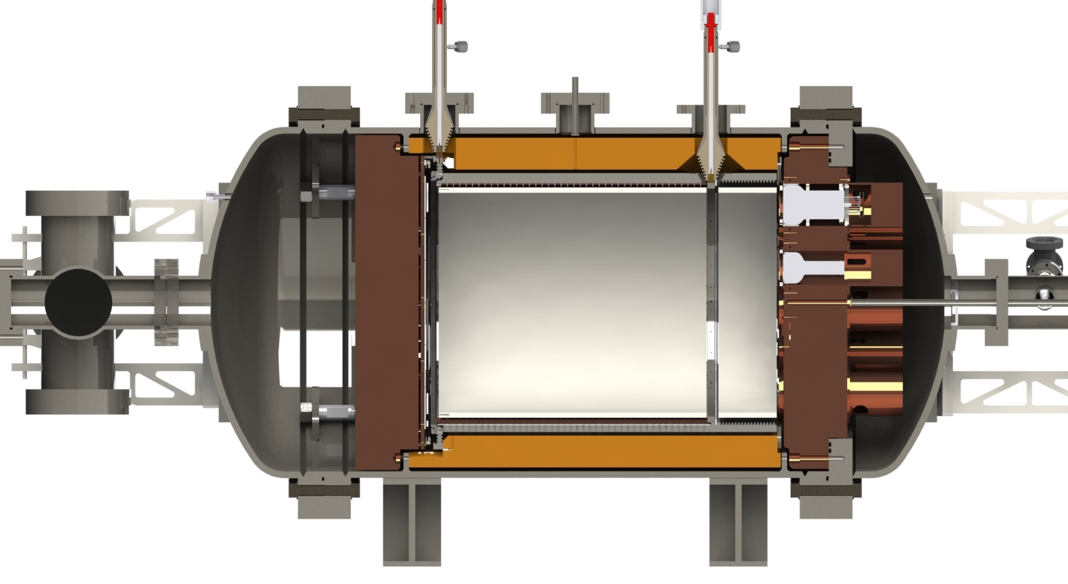
\includegraphics[height=8cm]{img2/NEWMay2016.png}
\caption{Top: a 3D drawing of the NEW detector, showing its main parts. Bottom: a lateral view of NEW, including the ancillary equipment used to extract the signals from the energy plane and the tracking plane.  } \label{fig:NewOverview}
\end{figure}

\begin{figure}[hpt!]
\centering
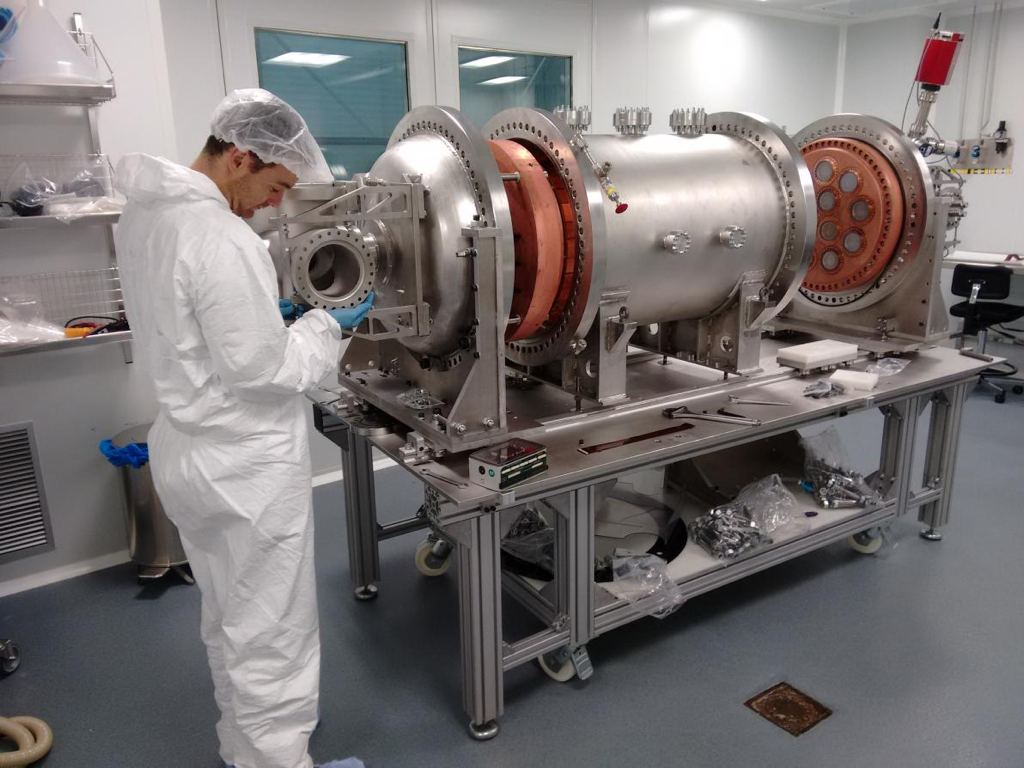
\includegraphics[height=7cm]{img2/NewInCRWIthAlberto.png}
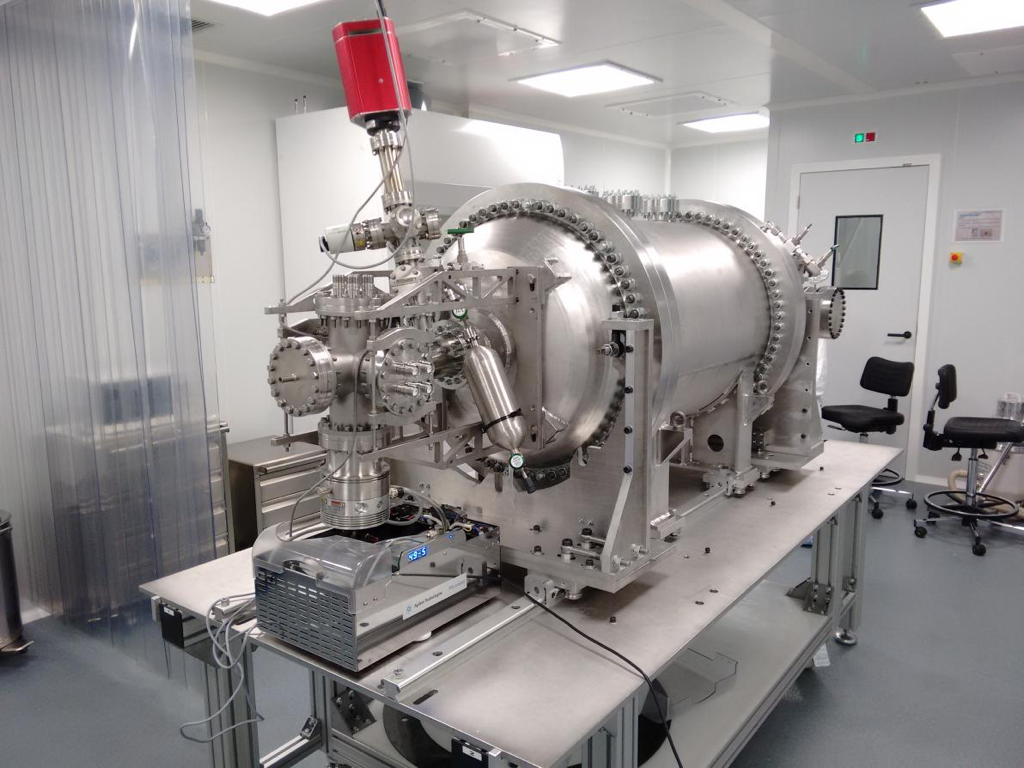
\includegraphics[height=7cm]{img2/NewSeenFromEP.png}
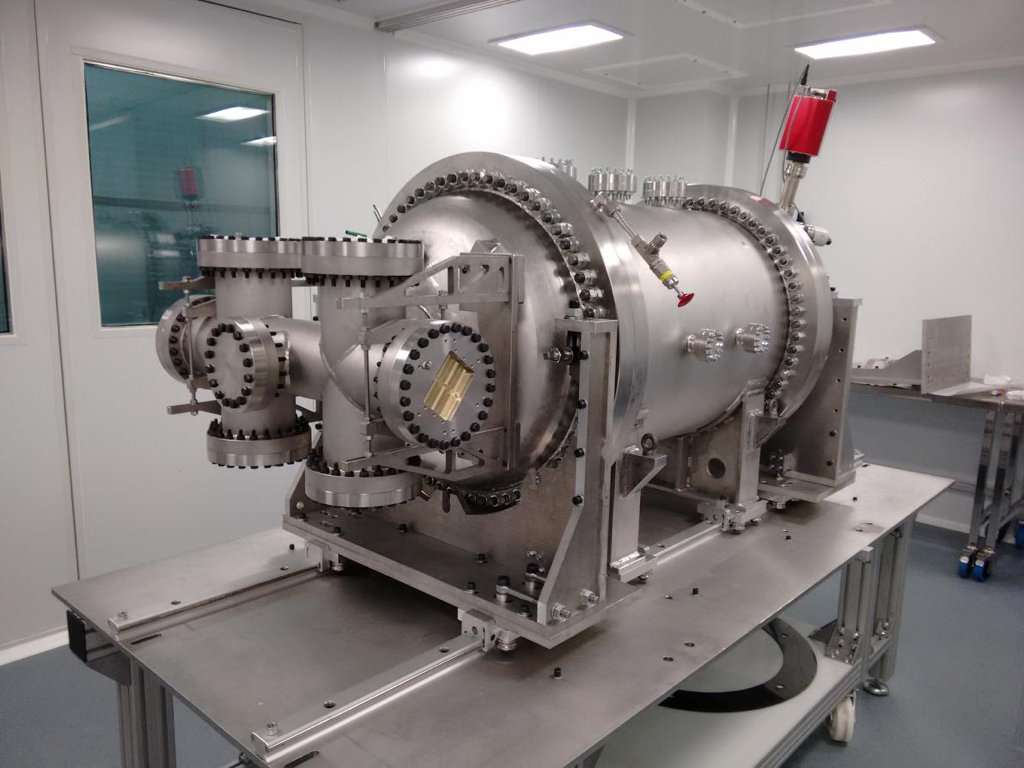
\includegraphics[height=7cm]{img2/NewSeenFromTP.png}

\caption{The NEW detector being assembled in the LSC clean room in 2015. Top: A picture from the side, showing the two end-caps open. The thick copper plates supporting the energy plane and the tracking plane are clearly visible. Middle: the detector seen from the Energy Plane side. The EP ``cross'' holds the feedthroughs (each cross side allows the extraction of 4 PMT signals) and also connects to the vacuum pump used to make vacuum in the vacuum side of the detector (in the picture the pump displays the level of vacuum achieved, $4.9 \times 10^{-5}$~mbar). The RGA is also clearly visible. Bottom. The detector seen from the tracking plane side. The TP ``spaceship" holds the TP feedthroughs.} \label{fig.New}
\end{figure}

The NEW detector, shown in figure \ref{fig:NewOverview} is the first stage of the NEXT experiment. The NEW pressure vessel  and field cage
 dimensions are roughly 1:2 with respect to those of NEXT-100. It deploys 20 \% of the NEXT-100 sensors and the xenon mass is about 10 kg at 15 bar. 

The primary goal of NEW is to provide an extra step in the construction of the NEXT-100 detector that allows the validation of the technological solutions proposed in the NEXT-100 technical design report (TDR)\cite{Alvarez:2012haa}. In addition, NEW will permit a measurement of the energy resolution at high energy, and the precise characterisation of the 2-electron topological signature, by measuring the \bbtnu\ mode. Last but not least, NEW will permit a realistic assessment of the NEXT background model before the construction of the NEXT-100 detector. 

Figure \ref{fig.New} shows the assembly of NEW at the LSC clean room during 2015. The detector has three main parts called {\em Energy Plane} (EP), {\em Tracking Plane} (TP) and {\em Field Cage} (FC). The EP and TP are already installed in the NEW pressure vessel. The FC will be installed during the first week of May 2016.

%\subsection{Pressure Vessel}
%The NPV has been manufactured by the company TRINOS vacuum system, with the same steel alloy selected for the NEXT-100 detector. The fabrication of the NPV was made possible, at zero cost for the NEXT collaboration, thanks to a CEDETI grant. Figure \ref{fig.npv} shows the pressure vessel and one of the torispherical heads. 
%
%\begin{figure}
%\begin{center}
%\includegraphics[width=0.80\textwidth]{img/NewPV.pdf}
%\includegraphics[width=0.80\textwidth]{img/NewPVHead.pdf}
%\end{center}
%\caption{\label{fig.npv} The NEW Pressure Vessel (NPV).}
%\end{figure}
%
%With an internal diameter of 64 cm and a length of 950 cm, the dimensions of the NPV are intermediate between NEXT-DEMO and NEXT-100. The NPV can hold pressures of up to 50 bar.
%
%\begin{figure}
%\centering
%\includegraphics[height=8cm]{img/PVInTable.pdf}
%\caption{The NEW detector: still a tabletop experiment.} \label{fig:PVInTable}
%\end{figure}
%
%Figure \ref{fig:PVInTable} shows the NPV sitting in a support platform. The platform will be first tested at IFIC, then moved to the LSC. The drawing illustrates the access to the detector. Each head has attached one of the photosensor detection systems (energy plane and tracking plane). 
%

\subsection{Energy Plane}
\begin{figure}[hpt!]
\centering
%\includegraphics[height=8cm]{img/NEPLateralView.pdf}
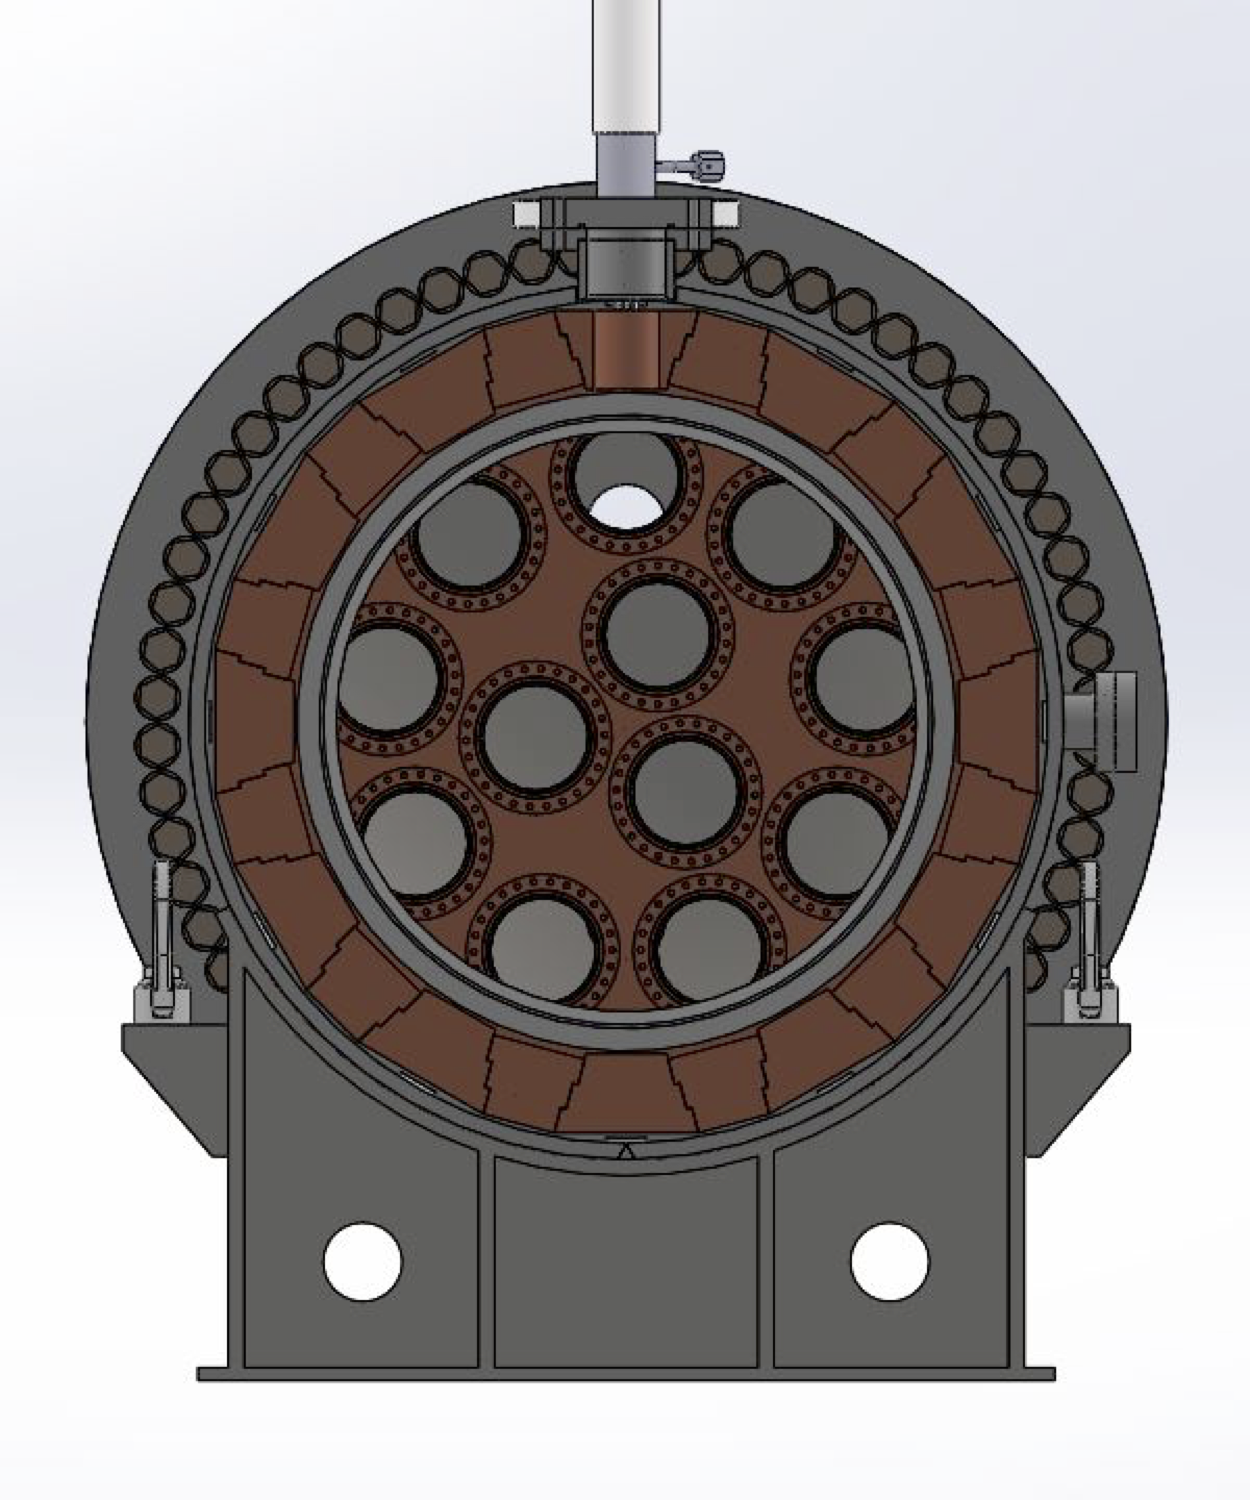
\includegraphics[height=8cm]{img2/NEPFrontView.png}
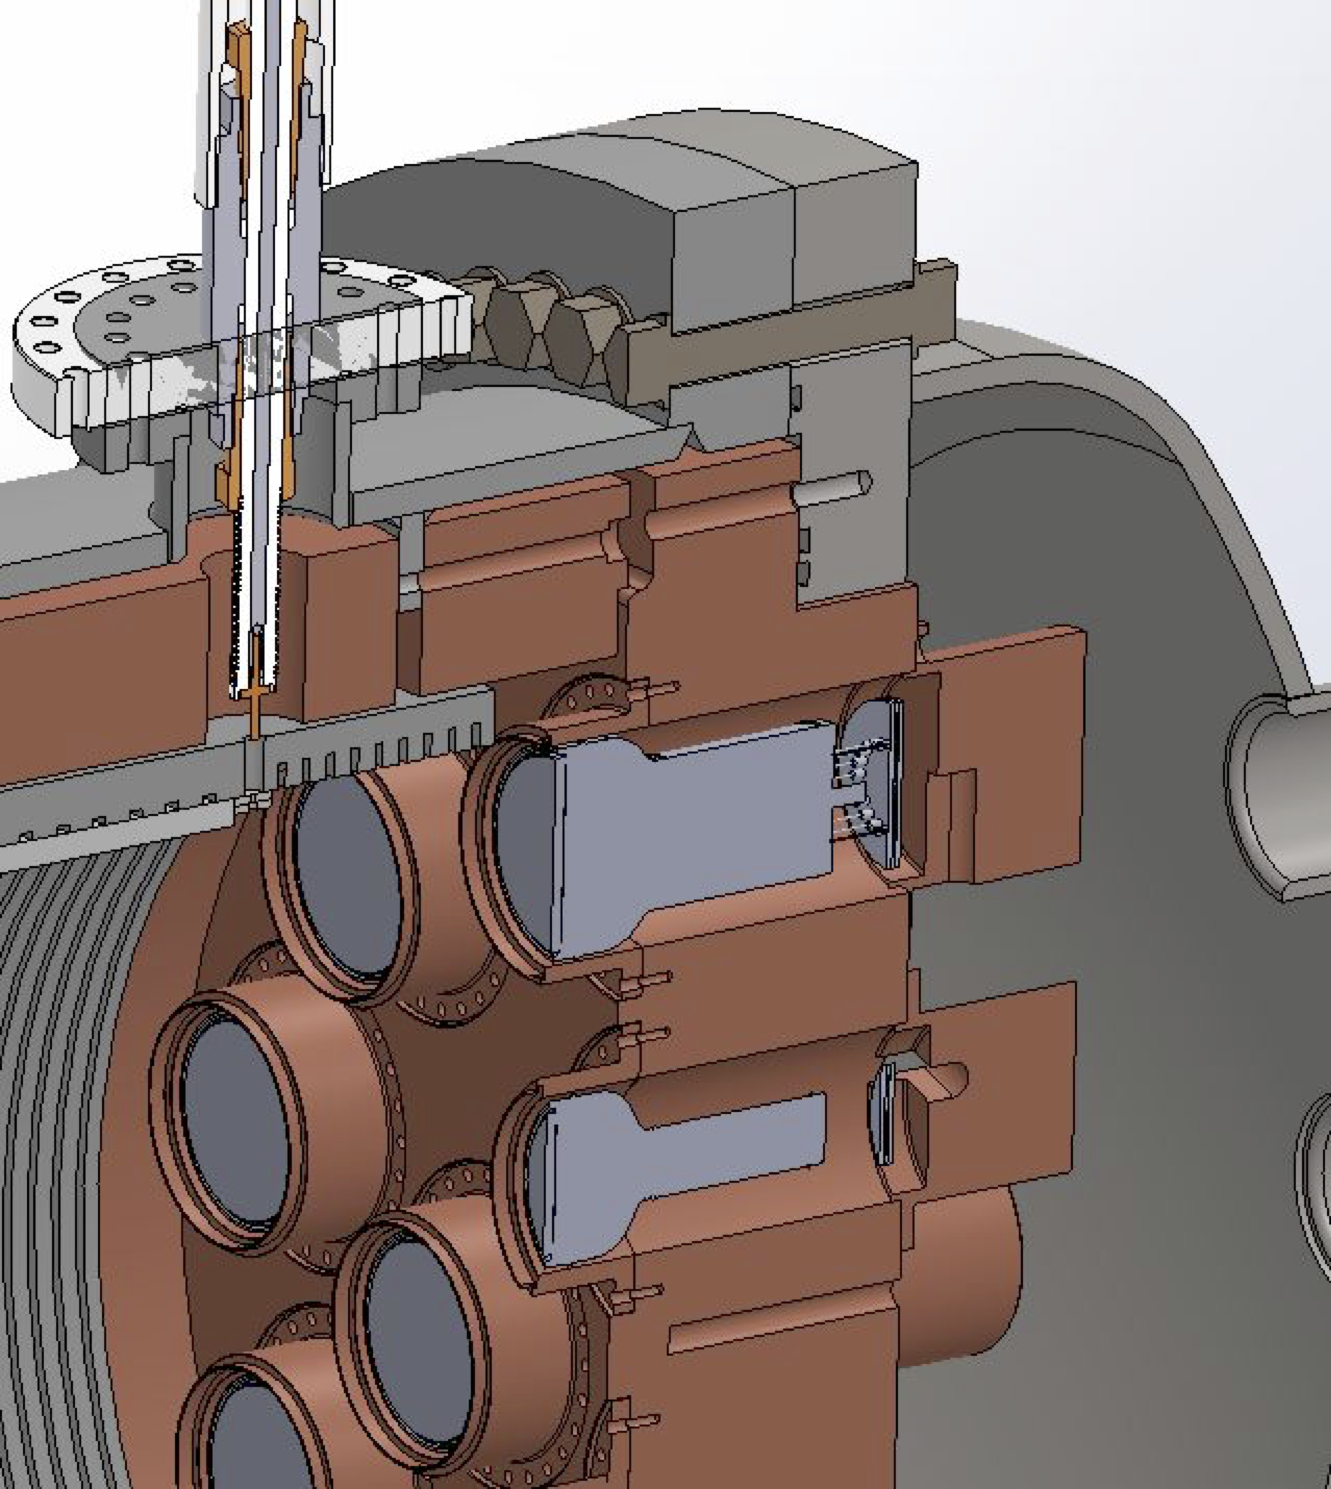
\includegraphics[height=8cm]{img2/NEPDetail.png}
\caption{The NEW energy plane (EP) deploying 12 PMTs operating in vacuum
and coupled to the field cage volume by sapphire windows coated with TPB. Top: front view. Bottom: Detail showing the sapphire windows and the PMT enclosures (aka cans) terminated in thick copper caps for radiation shielding.} \label{fig:NEP}
\end{figure}


\begin{figure}[hpt!]
\centering
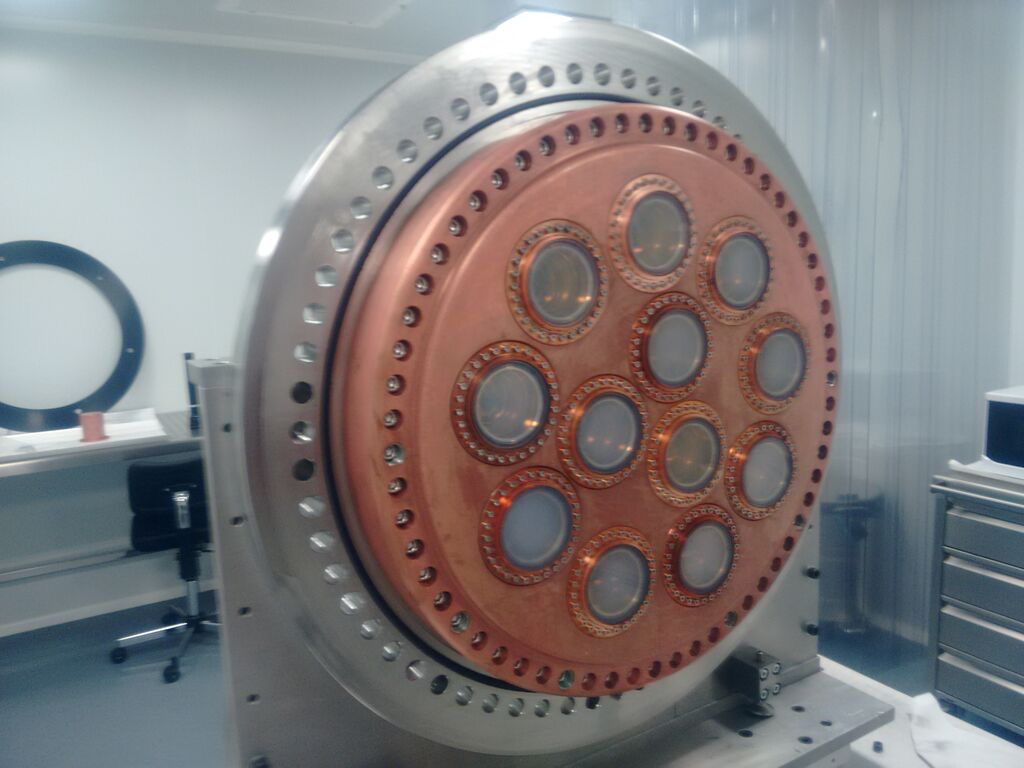
\includegraphics[height=8cm]{img2/EP_ENDCUP.png}
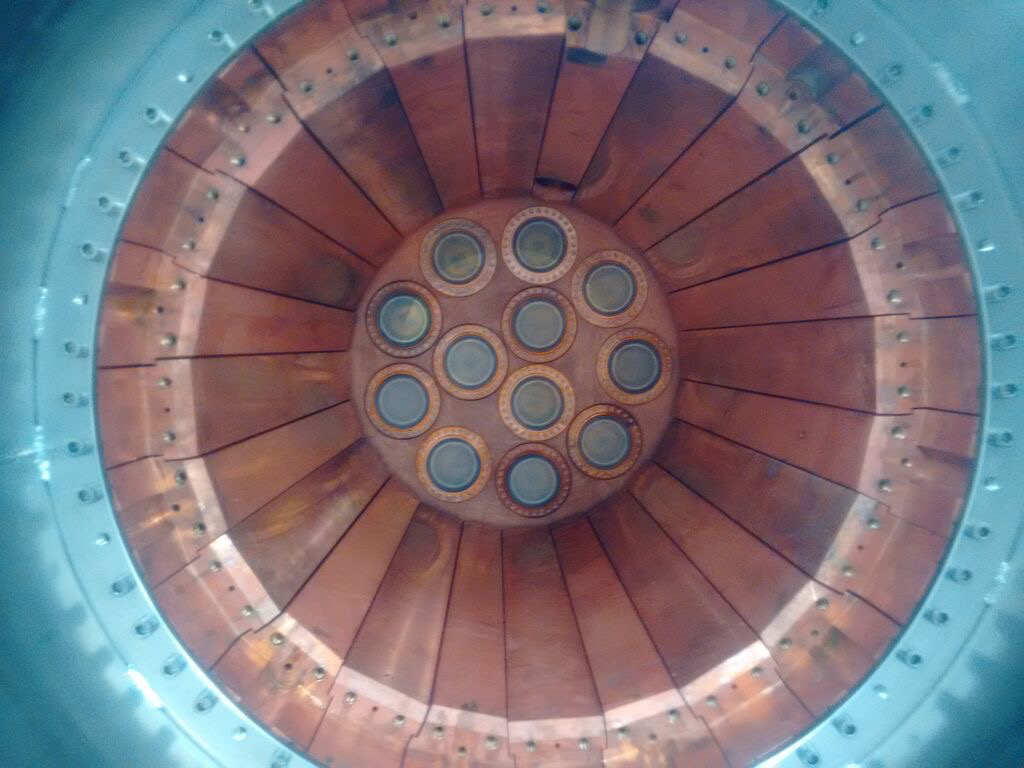
\includegraphics[height=8cm]{img2/EPI.png}
\caption{Assembly of the EP in 2015. Top: The end-cup plate (mother-can) with the sapphire windows already installed. Bottom: the energy plane seen from the tracking plane side. The picture also shows the cooper bars from the inner copper shielding, intended to attenuate the external radiation. } \label{fig.EPA}
\end{figure}

The energy plane is shown in figure \ref{fig:NEP} and pictures of the installation in 2015 are shown in
figure \ref{fig.EPA}. The EP 
consists of a 11 cm thick copper support plate (called mother-can) with 12 copper window
covered with brazed sapphire windows fixed to the front of the plate. The
set-up as a whole seals the pressure vessel from the PMT-region,
which is held at vacuum levels of
$<10^{-5}$~mbar. Additional copper shielding fixed to the
vacuum side of the apertures, offer further shielding against gammas traversing the PMTs and
entering in the detector volume. The 12 Hamamatsu R11410 PMTs are optically coupled to 
the sapphire window using NyoGel OCK-451. The sensors are held in place by a plastic brace and spring.

The PMTs receive high voltage and have their signal extracted via a
shielded twisted pair cable connected to a feedthrough in the energy-plane head. The distribution of
signal and supply at each individual PMT is controlled via a
Kapton circuit board (base), covered with a
copper cap filled with epoxy and connected to the support plate. The cap acts as a heat sink.


\subsection{Tracking Plane}

\begin{figure}[hpt!]
\centering
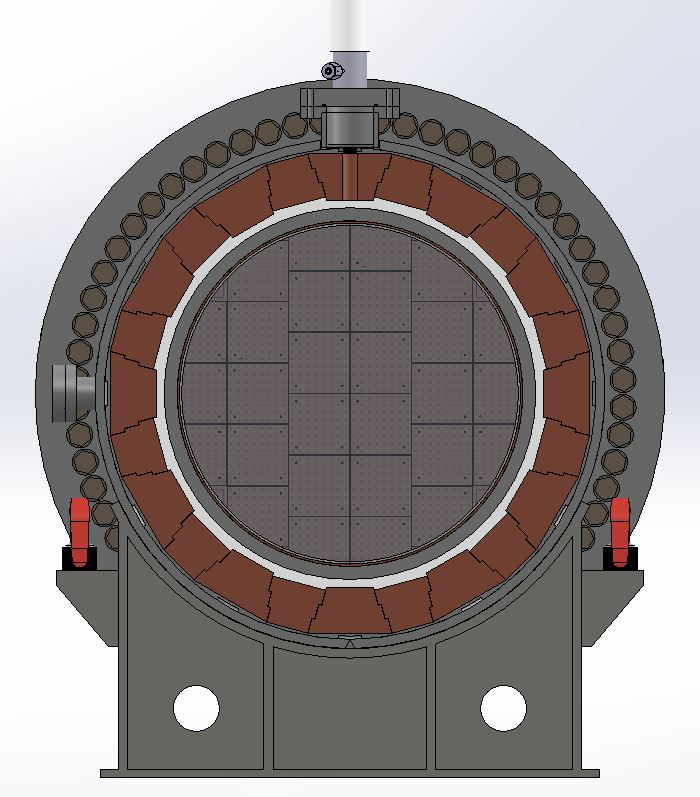
\includegraphics[height=8cm]{img2/TrackingPlane.png}
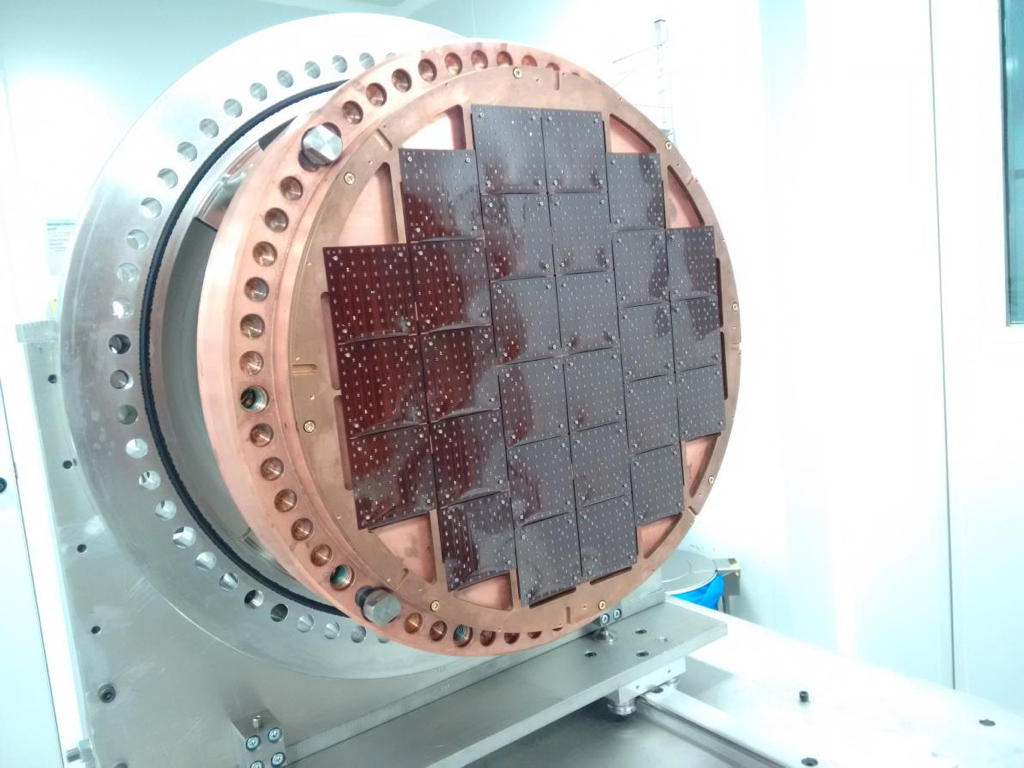
\includegraphics[height=8cm]{img2/TPI1.png}
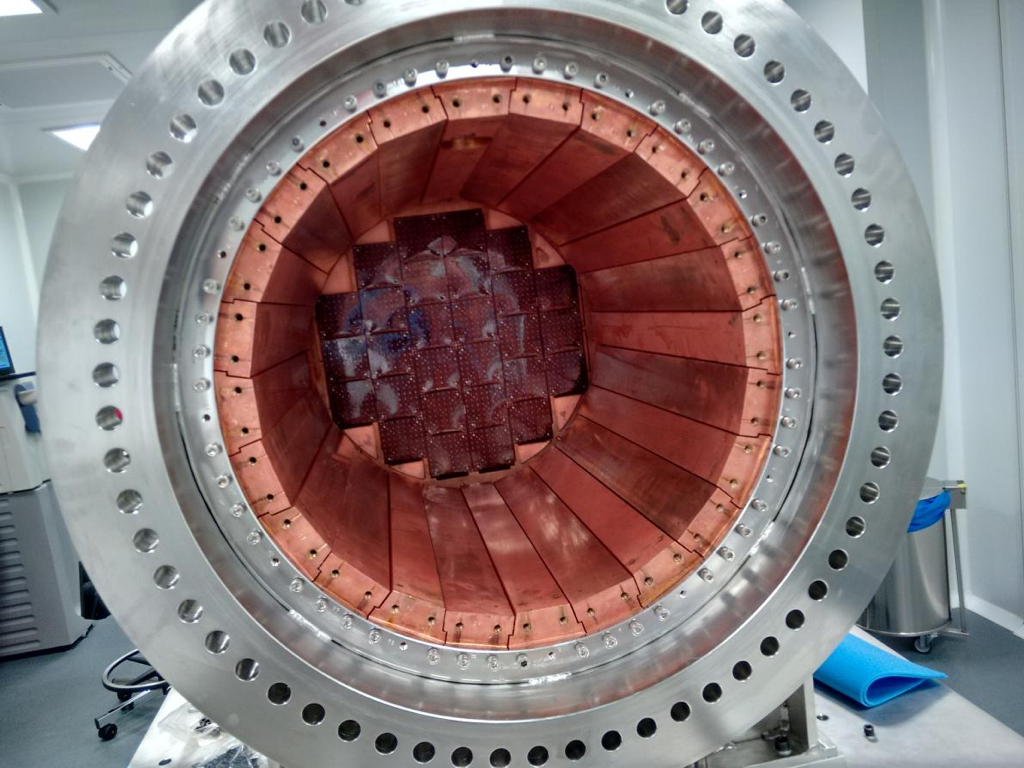
\includegraphics[height=8cm]{img2/TrackingPlaneFromEP.png}

\caption{The NEW tracking plane. Top: A drawing, showing the KDBs over-covering the fiducial area;.
Middle: The KDBs installed in the TP support plate. Bottom: The TP seen from the EP side.} \label{fig:NTP}
\end{figure}

The NEW tracking plane, shown in figure \ref{fig:NTP} permits the reconstruction of the trajectories of charged particles, (e.g., electrons), in the NEW/NEXT detectors. It consists of a matrix of silicon photomultipliers (SiPMs) which operate as light pixels, providing a 2D picture of the event (the third coordinate is given by the drift time). The SiPMs are radiopure 1-mm sensors, manufactured by SENSL. The TP is made of 28 radiopure circuits called Kapton DICE-Boards (KDB). Each KDB has an $8\times8$~ SiPM array, where each SiPM is placed at a 1-cm pitch. Each KDB also includes a NTC temperature sensor and one LED for calibration. The KDBs over-cover the fiducial region with $\sim$1800 SiPMs, ensuring that there are no dead regions. The connector is located at the end of a long tail, and is screened from the gas, in the fiducial volume, by a 120 mm thick copper shield.

%\subsubsection*{Silicon photomultipliers}\label{sec:sipms}
%A Silicon PhotoMultiplier (SiPM) consists of a matrix of photodiodes (diode which converts light into current), operating in Geiger mode. These photodiodes are connected in parallel becoming each one a pixel of the SiPM. A detailed picture of this structure is shown in figure~\ref{fig:sipm}. The pixels are connected by aluminum stripes to read out the combined signals, which is the sum of all pixels. The pixels are electrically decoupled by polysilicon resistive stripes between the pixels. 
%
%The SiPM used in the NEW detector are the SensL MicroFC-10035-SMT-GP model. This model has demonstrated to be sufficiently radiopure to operate in a low background experiment and also its dark current ($\sim100kHz/mm^2$) is much lower than in the previous models, allowing for easier calibration and an improved threshold for low energy events.
%
%
%\begin{figure}[hpt!]
%  \centering
%  \subfloat[\textit{Detail of the pixel array}]{%\label{fig:cabling:}
%  \includegraphics[height=0.22\textwidth]{TrackingPlane/IMG/PixelMatrix.pdf}}   
%  \hspace{5mm}             
%  \subfloat[\textit{Hamamatsu SiPM}]{%\label{fig:ad:ads7883}
%  \includegraphics[height=0.22\textwidth]{TrackingPlane/IMG/sipm.jpg}}
%  \hspace{5mm}             
%  \subfloat[\textit{SiPM from SensL}]{%\label{fig:ad:ads7883}
%  \includegraphics[height=0.22\textwidth]{TrackingPlane/IMG/sensl.jpg}}
%  \caption{\textit{Silicon photomultipliers}}
%  \label{fig:sipm}
%\end{figure}
%

\subsubsection*{KDB arrangement and cabling}
\label{sec:DB}

A scheme of the TP cabling is shown in 
figure \ref{fig:cabling:scheme}). The engineering problems that had to be solved were: a) to place connectors behind the copper shielding; b) to pass the KDB analog signals through custom feedthroughs; c) to transport the signals to the front-end electronics, via long-cables.  

\begin{figure}[hpt!]
    \bigskip
    \begin{center}\leavevmode
        \rotatebox{0}{
        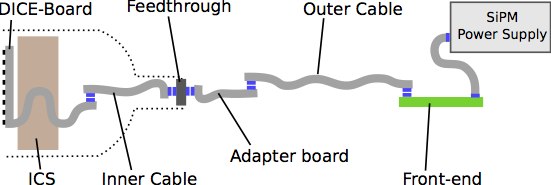
\includegraphics[width=.8\textwidth]{img2/Simple.png}}
        \caption{\textit{Tracking plane cabling scheme.}}
        \label{fig:cabling:scheme}
    \end{center}
\end{figure}



%Fig. \ref{fig:spring_detail} shows the detail of one of those springs.

%\begin{figure}[h!]
%\begin{center}
%\includegraphics[width=0.45\textwidth]{TrackingPlane/IMG/spring_plate_detail}
%%\hspace{15mm}
%%\includegraphics[width=0.39\textwidth]{IMG/DB.JPG}
%\caption{Detail of one of the springs in the tracking plane thin plate that will allow to accommodate the tracking plane perfectly parallel to the electroluminescence region.}
%\label{fig:spring_detail}
%\end{center}
%\end{figure}


\begin{figure}[hpt!]
\begin{center}
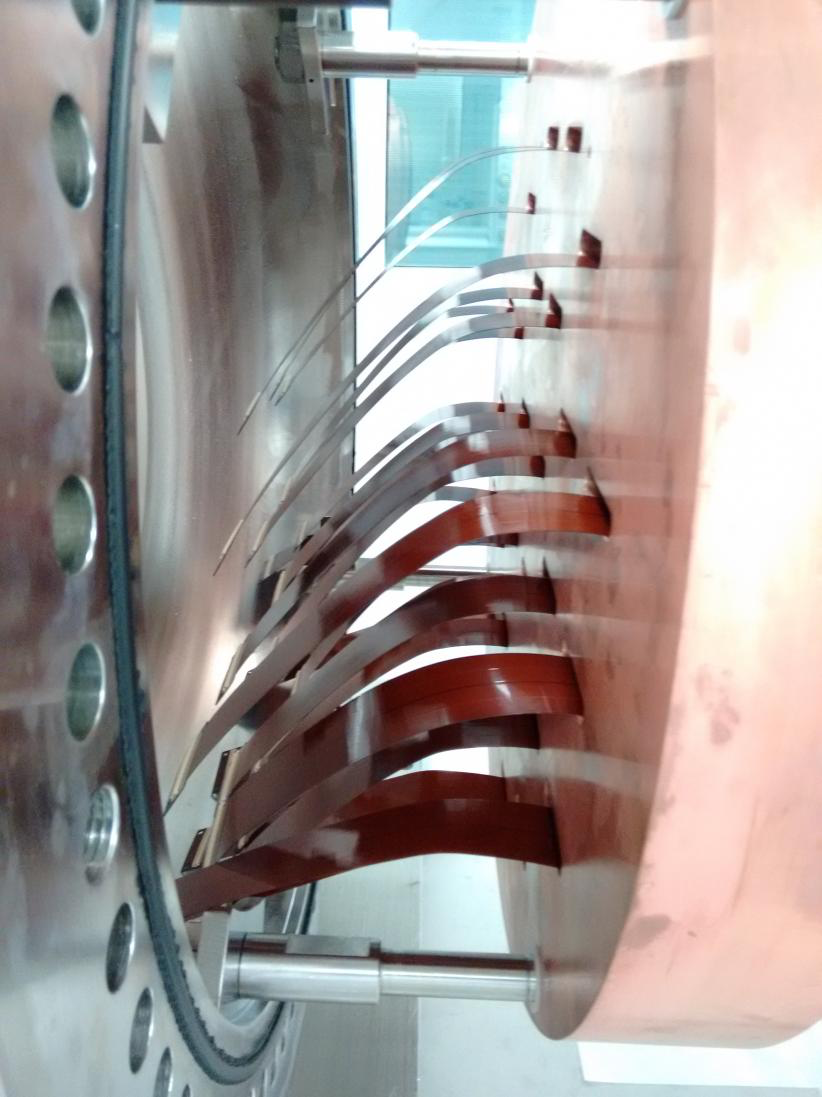
\includegraphics[width=8cm]{img2/cabling.png}
\caption{Dice-Boards cables passing through the holes in the shielding plate. At the end of the tail there is a connector that will allow for an extension of the cable to reach the feedthrough.}
\label{fig:cabling}
\end{center}
\end{figure}

\begin{figure}[hpt!]
\begin{center}
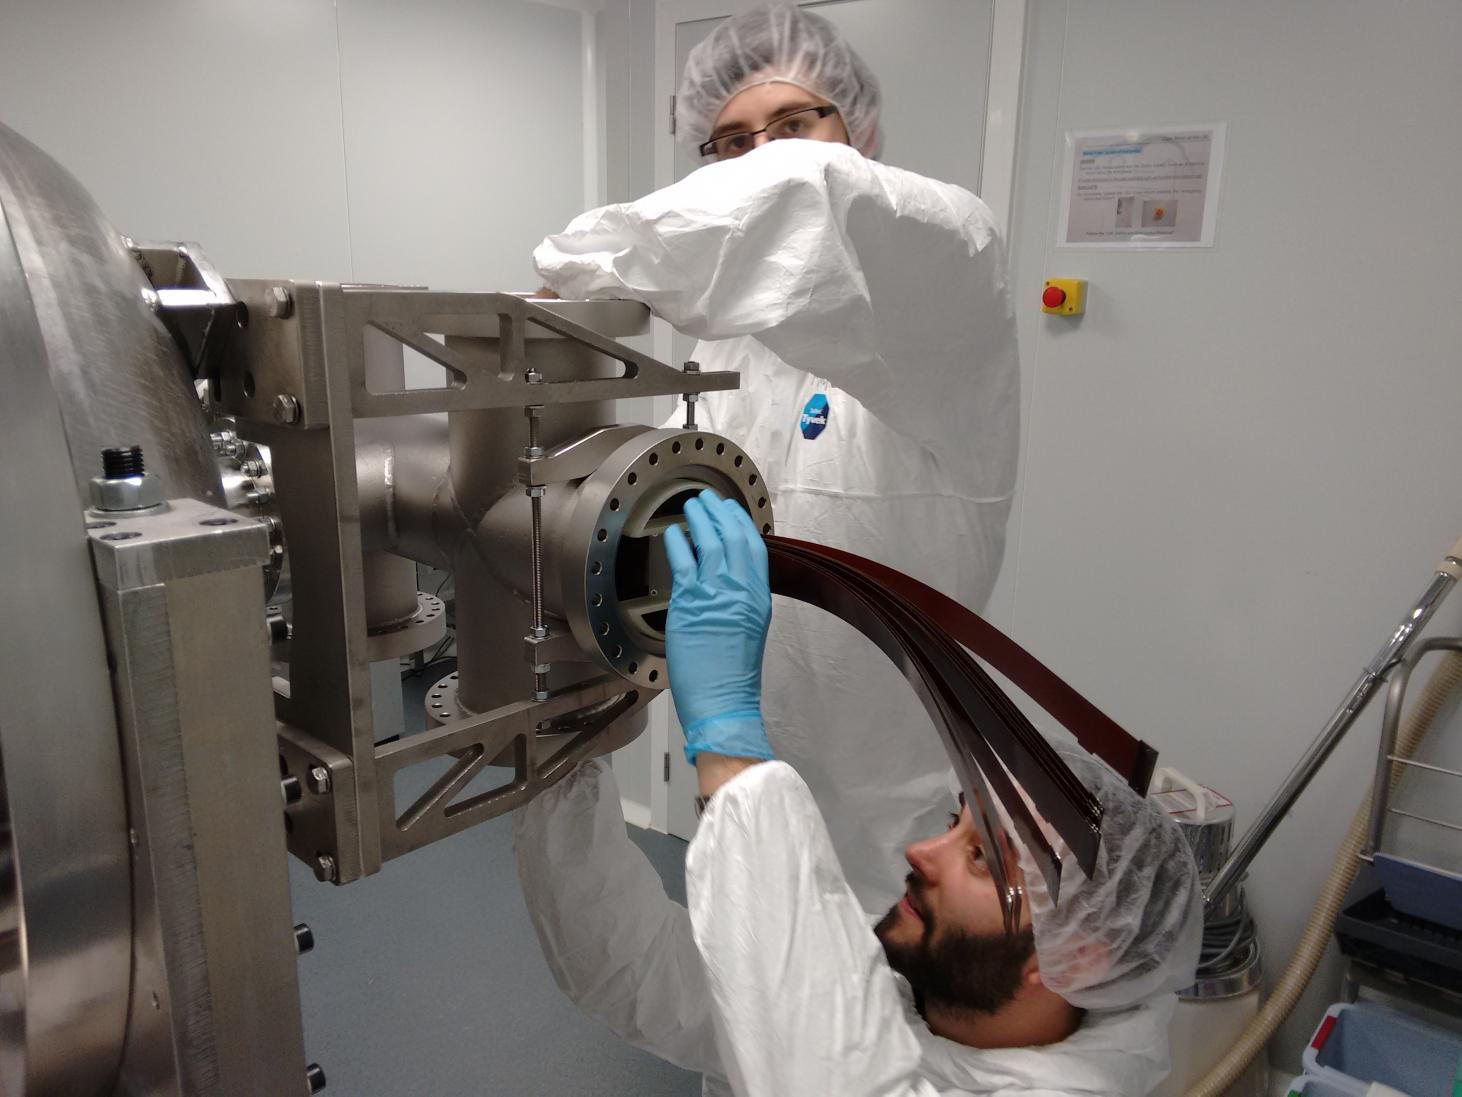
\includegraphics[width=12cm]{img2/cabling_spaceship.png}
%\includegraphics[width=0.45\textwidth]{TrackingPlane/IMG/spacechip_cabling}
%\includegraphics[width=0.45\textwidth]{TrackingPlane/IMG/spaceship_unmounted}
\caption{Cables being extracted from the ``spaceship'' during TP assembly, at the LSC clean room.}
\label{fig:cabling_spaceship}
\end{center}
\end{figure}

The KDBs  where mounted on top of a thin plate of copper held by springs to the main copper plate that acts as a shielding. The reason of those springs is that they will allow for a small movement of the plate during the assembly and when closing the detector allowing for a perfect match of the tracking plane with the EL region. 

Once the KDBs are mounted the tail has to be passed through the holes in the shielding plate 
(figure \ref{fig:cabling_spaceship}). At the end of the tail a connector is soldered to plug a cable extension made of the same materials than the DICE-Boards. Those cables have to be organised to reach 5 different feed-throughs. The distribution of the cables is done using 3D printed structures placed inside a steel structure that will allow to extract the SiPMs cables and also is the point where the piping for vacuum and evacuation connects.


The final step in the connection of inner cables of the tacking plane is the connexion to the tracking-plane feedthroughs (TPFT). Each one of these custom-made FT allows up to 6 KDB connexions. Extracting the signals of the 29 KDBs require then  5 TPFT. Figure \ref{fig:TPFT} shows the front and the back side of theTPFT as well as the cable connexion.

\begin{figure}[hpt!]
\centering
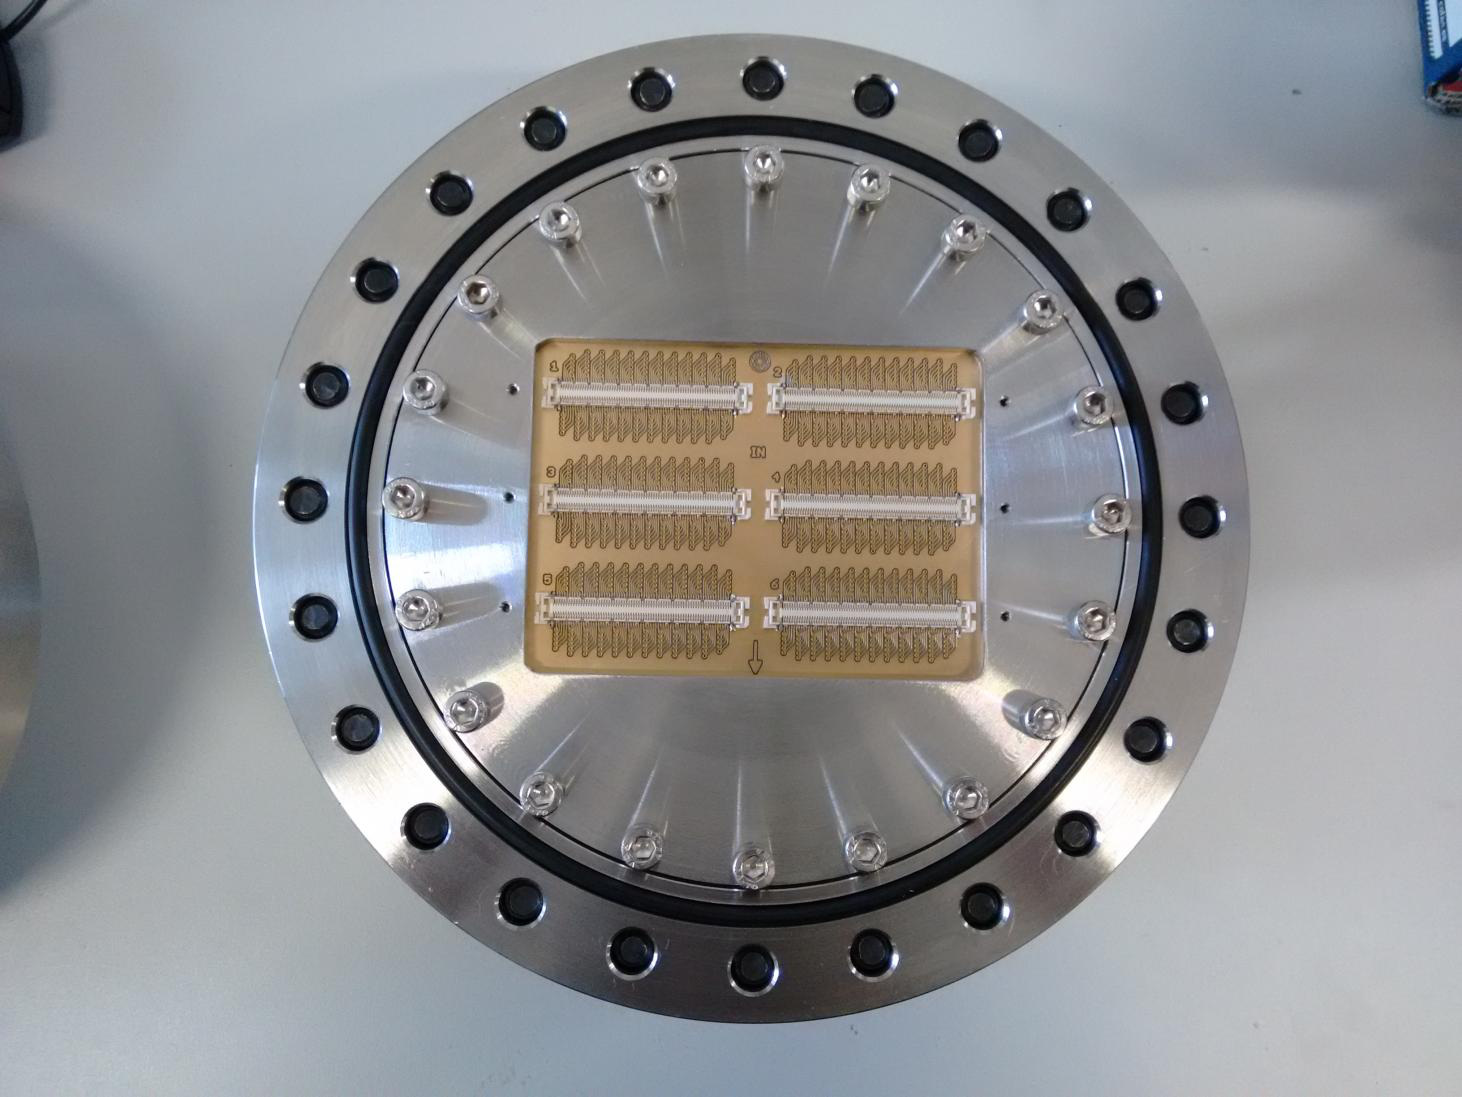
\includegraphics[width=0.45\textwidth]{img2/TPFT1.png}
%\includegraphics[width=0.45\textwidth]{TrackingPlane/IMG/TPFT2}
%\includegraphics[width=0.45\textwidth]{img/TPFTI.png}
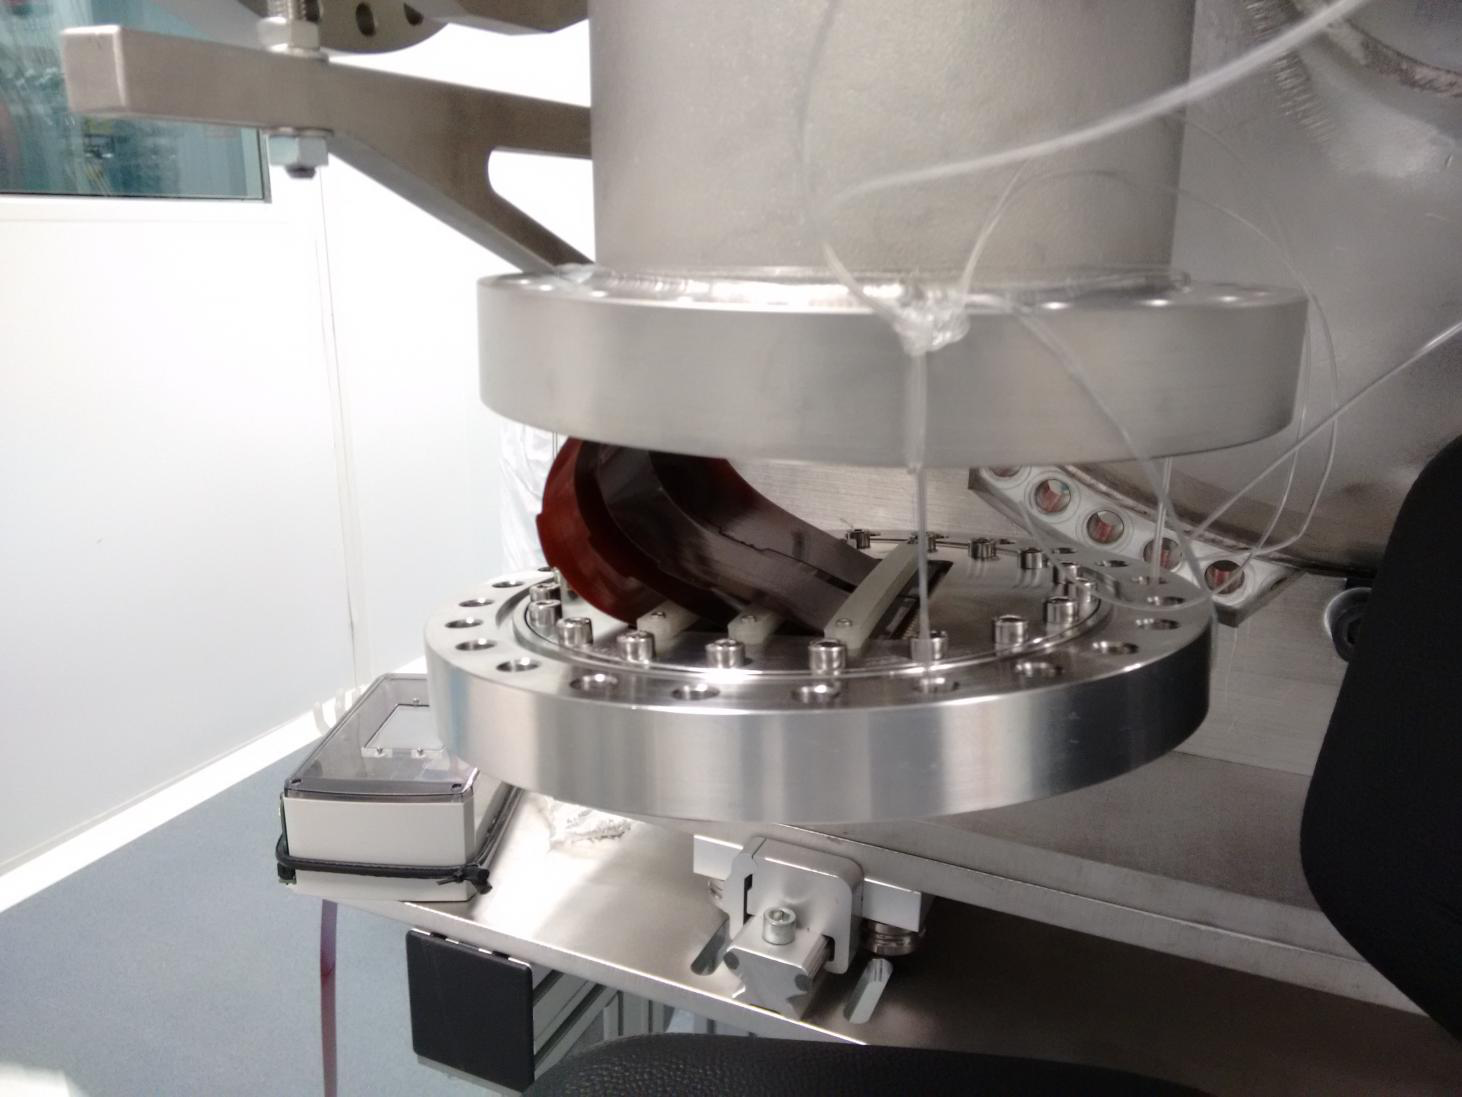
\includegraphics[width=0.45\textwidth]{img2/TPFT_connected.png}
\caption{The tracking-plane feedthroughs (TPFT). Left: Inner side of the TPFT. Right: Cable connexion.}
\label{fig:TPFT}
\end{figure}


\subsubsection*{External cabling}\label{sec:ext}


\begin{figure}[hpt!]
\centering
\includegraphics[width=.45\textwidth]{img2/KrakenInLC.png}
\includegraphics[width=.45\textwidth]{img2/krakenOutOfLC.png}
%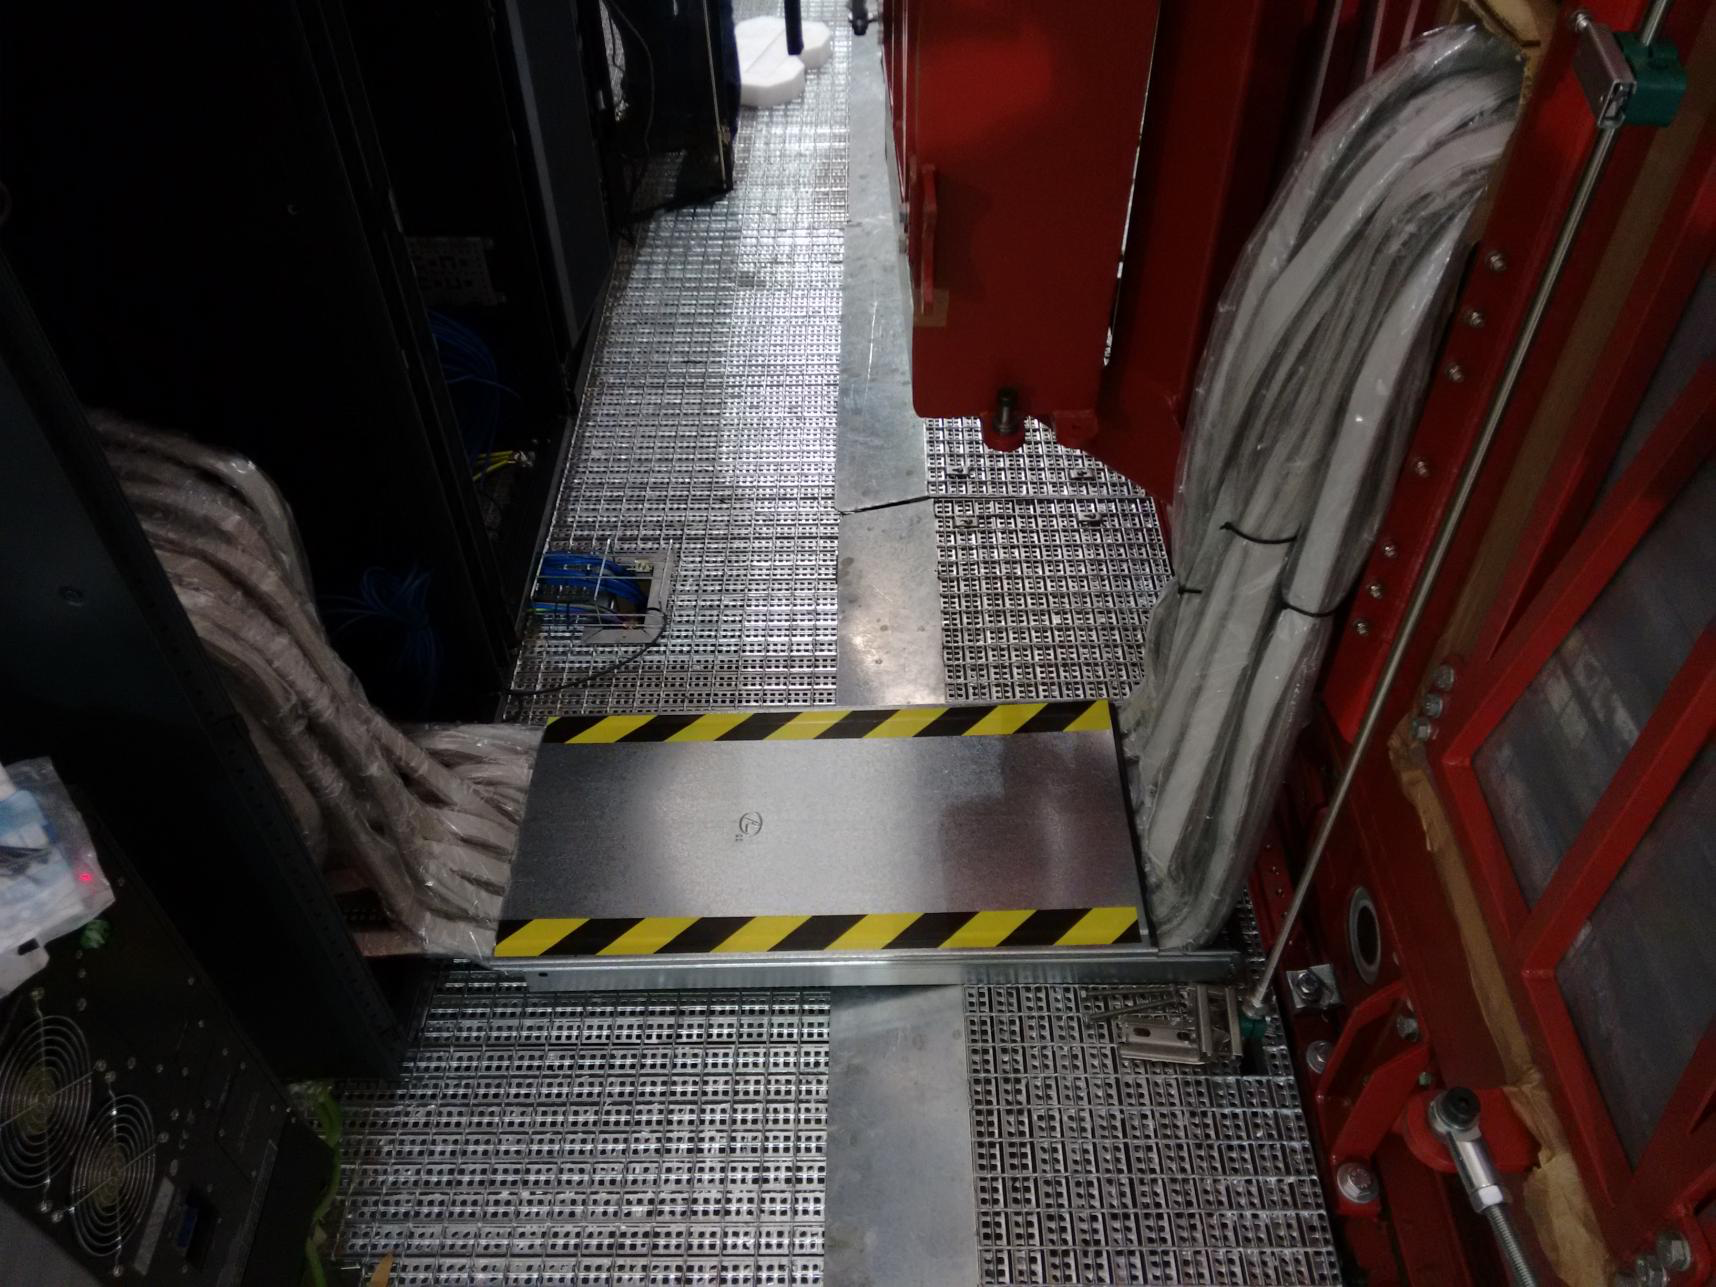
\includegraphics[width=.45\textwidth]{img2/cabling_under_platform.png}
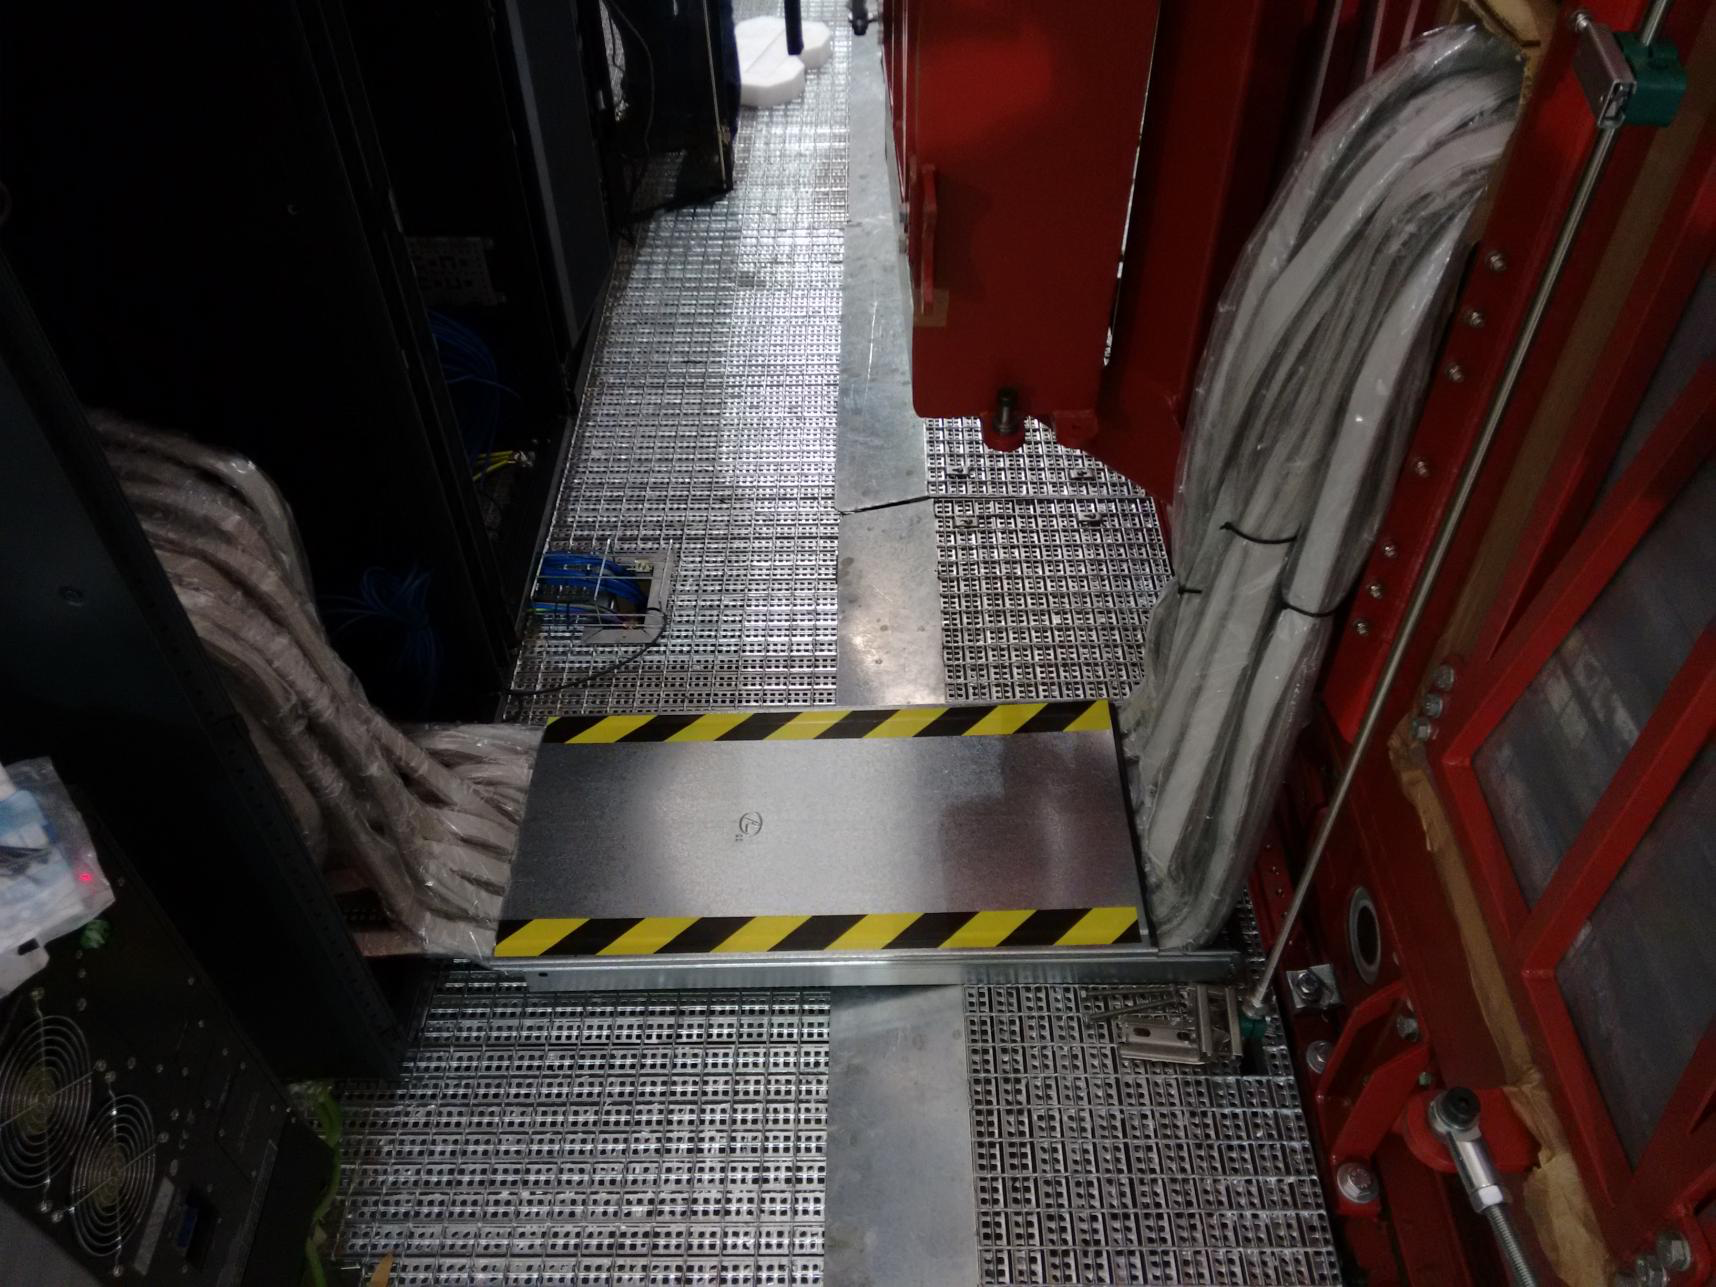
\includegraphics[width=.45\textwidth]{img2/cabling_under_platform.png}
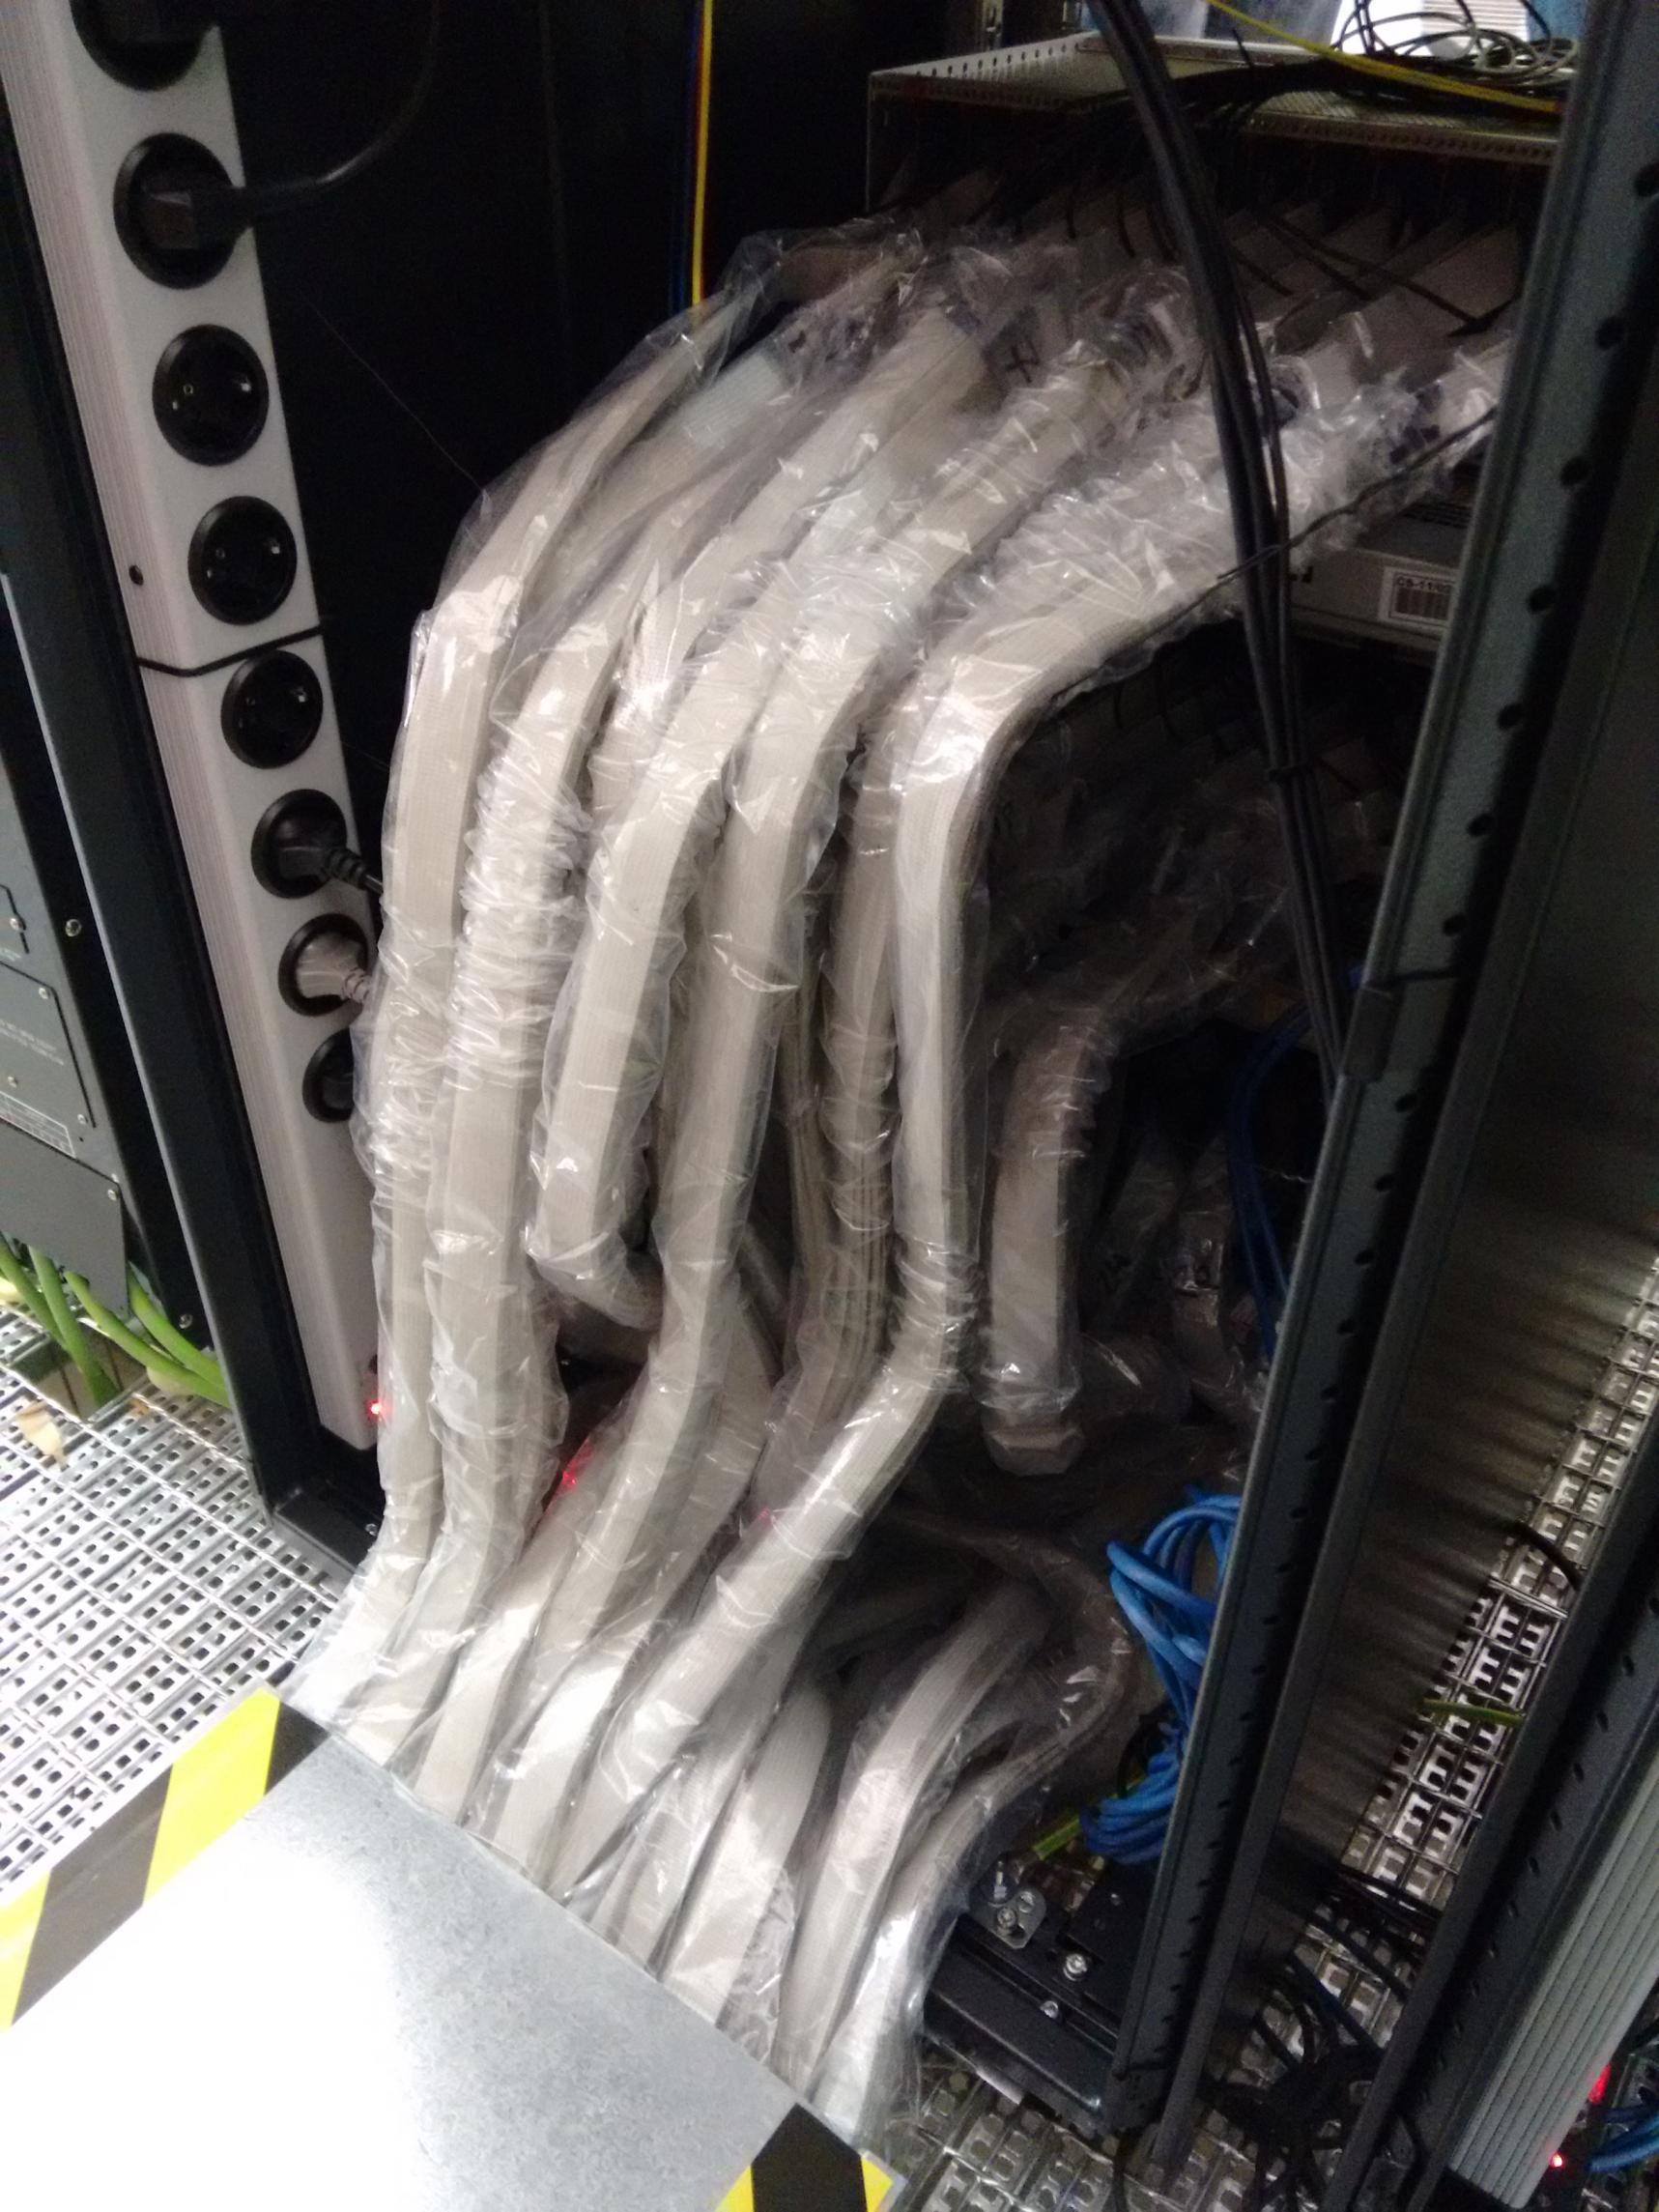
\includegraphics[width=.45\textwidth]{img2/cabling2FEE.png}
\caption{Different parts of the external cabling of the tracking plane. Up left shows the cables being directed to the exit hole of the lead castle. Up right shows the cables coming out of the lead castle. Bottom left shows how the cables move under the platform. Bottom right shows a detail of the connexion of the cables to the FEE boards.}
\label{fig:external_installation}
\end{figure}

In order to keep background events to a minimum, front-end electronics are placed nearby the detector but beyond the lead castle that surrounds the TPC, with a total cable length of $\sim$ 5 m from the sensor to the electronics. This poses a challenge in the design of a cabling solution that (1) is radio-clean enough to be inside the detector, (2) keeps enough signal-to-noise ratio in the relevant signal bandwidth for the gated integrator with a 5 m cable, (3) is cost-effective, (4) includes SiPM biasing voltage wires and (5) is also valid for the final NEXT phase (NEXT-100).

Differential transmission lines on fine-pitch FFC cables outside the detector were chosen as a good trade off between performance and cost. As shown in figure \ref{fig:external}, the cables are 0.5 mm pitch with $280 \times 76 \mu$m traces embedded in a thin polyester layer. The anode and the cathode of each SiPM are connected to the \textit{signal} and \textit{bias} lines respectively. Channels are separated by a guard trace connected to the analog ground in the front-end. Therefore three lines are needed for each SiPM channel. In addition, each KDB adds several more lines, for the  temperature sensor and  calibrating LEDs.

%\begin{figure}[hpt!]
%\centering
%\includegraphics[width=.6\textwidth]{TrackingPlane/IMG/section.pdf}
%\caption{Cross-section of the external cable (just two channels are shown).}
%\label{fig:external}
%\end{figure}

Since commercial cables with the required density of traces were not available, the adopted solution was to split into four FFC cables. This way, the signals of a whole DICE-Board are distributed in four cables of 51 wires each. This distribution is done just at the output of the feedthrough, using a Kapton adapter board. This board has the same stackup as the DICE-Board or the inner cable, and splits the signals in four \textit{DF9 Hirose} connectors for the long cables.

In order to further reduce the noise coupled to the external cables, they are wrapped with a 1 mm aperture mesh, also connected to the analog ground at the front-end. This mesh is has its maximum attenuation rated at 1 MHz, which covers the range of frequencies we want to attenuate.

The external cables cables have been connected to the output of the TPFT and then they go below the platform until the position of the FEE boards where they are connected, as shown in figure \ref{fig:external_installation}.

%\subsubsection*{Sensor characterisation}
%The simplest method to calibrate the SiPMs is shown in figure \ref{fig:calibration} (top panel), and consists  in finding the different peaks associated to the different photoelectron numbers in the SiPM and extract the gain according to their separation. The first results from NEW show that the gain spread among the SiPMs is very small (figure \ref{fig:calibration} bottom).
%%The first data extracted from the tracking plane has been used to make a first evaluation of the behaviour of the different sensors and DICE boards. The SiPMs have been tested with no light (only dark counts were recorded) and with light pulses from the blue LEDs installed in the energy plane (Fig. \ref{fig:calibration} bottom).
%
%\begin{figure}[hpt!]
%\centering
%\includegraphics[width=0.45\textwidth]{TrackingPlane/IMG/normal_calibration}
%\includegraphics[width=0.45\textwidth]{TrackingPlane/IMG/SIPMsGain}
%%\includegraphics[width=0.45\textwidth]{IMG/SiPM_LED_noLED}
%\caption{Top: standard method for calibration where the charge corresponding to the different number of photoelectrons in the SiPMs is estimated with a fit to the peak. The gain of the SiPM is calculated using the separation of the different peaks. Bottom: Histogram showing the gain of all the SiPMs in the plane. This histogram shows that the spread on the SiPMs gain is only of the order of a few ADC counts. 
%%Bottom: Comparison of two spectra from the same SiPM, with (blue) and without light (red).
%}
%\label{fig:calibration}
%\end{figure}

\subsubsection*{Reflectors}

The material of choice for the KDBs (Kapton) as many advantages including flexibility, little degassing and radiopurity. However it is a poor reflector. In order to increase the amount of light recorded by the energy plane, a 2 mm teflon reflector is placed in front of each KDB. The reflectors (figure \ref{fig:reflector}) have holes to accommodate the SiPMs without damaging them and also have a space for the thermal sensor and the LEDs. However no holes are necessary for the LEDs, since teflon is sufficiently transparent to the blue light they emit. 
\begin{figure}[hpt!]
\centering
%\includegraphics[width=0.45\textwidth]{TrackingPlane/IMG/teflon1}
\includegraphics[width=0.45\textwidth]{img2/teflon2.png}
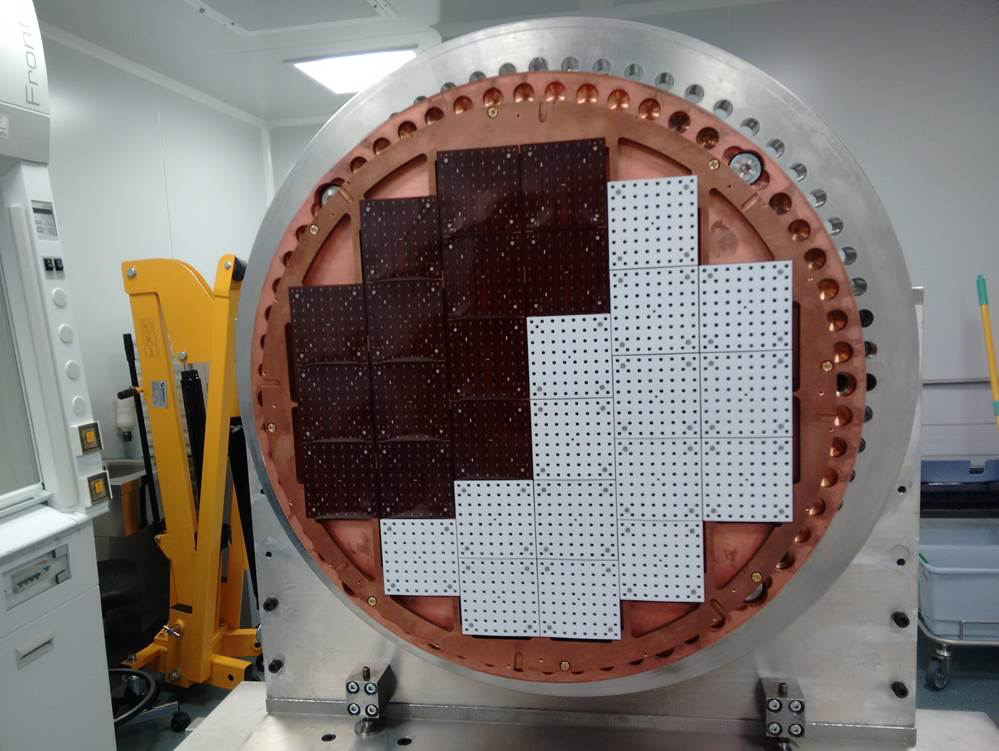
\includegraphics[width=0.45\textwidth]{img2/HalfAndHalf.png}

\caption{Top: Front side (EL) of the reflector. Bottom: The TP with half covered with the reflectors.}
\label{fig:reflector}
\end{figure}

%\subsection{The front-end electronics and DAQ} 
%
%%%%%%%%%%%
%\begin{figure}
%\centering
%\includegraphics[width=0.7\paperwidth]{img/FEE_SiPM.pdf}
%\caption{\small Functional blocks in the FEB card.}
%\label{fig:feb}
%\end{figure}
%
%The front-end electronics for the PMTs in NEW and NEXT-100 will be very similar to the system developed for the NEXT-DEMO prototype. The first step in the chain is to shape and filter the fast signals produced by the PMTs to match the digitiser and eliminate the high frequency noise. An integrator is implemented by simply adding a capacitor and a resistor to the PMT base. The charge integration capacitor shunting the anode stretches the pulse and reduces the primary signal peak voltage accordingly.
%
%The electronics for the SiPMs is very simple. Our design consists of a  64 channel Front-End Board (FEB, Figure~\ref{fig:feb}). Each FEB takes the input of a single DB (transmitted via low-crosstalk kapton flat cables) and includes the analog stages, ADC converters, voltage regulators and an FPGA that handles, formats, buffers and transmits data to the  DAQ. 
%
%The NEW and NEXT-100 data-acquisition systems (DAQ) follow a modular architecture named the Scalable Readout System (SRS), already described in our CDR \cite{Alvarez:2011my}. At the top of the hierarchy, a PC farm running the DAQ software, DATE, receives event data from the DAQ modules via Gigabit Ethernet (GbE) links. The DATE PCs (Local Data Concentrators, LDCs) assemble incoming fragments into sub-events, which are sent to one or more additional PCs (Global Data Concentrators, GDC). The GDCs build complete events and store them to disk for offline analysis.
%
%The DAQ modules used are Front-End Concentrator (FEC) cards, which serve as the generic interface between the DAQ system and application-specific front-end modules. The FEC module can interface different kinds of front-end electronics by using the appropriate plug-in card. The FEC card and the overall SRS concept have been developed within the framework of the CERN RD-51 collaboration. 

\subsection{Field Cage}

%\begin{figure}[hpt!]
%\centering
%\includegraphics[height=8cm]{img/NFC.pdf}
%\caption{The NEW field cage (NFC).} \label{fig:NFC}
%\end{figure}

\begin{figure}[hpt!]
\centering
\includegraphics[height=8cm]{img2/FieldCageWithRing.png}
\caption{Detail of the copper rings in the drift region.} \label{fig:drift1}
\end{figure}

The goal of the FC is to provide an homogeneous and uniform electric field inside the active volume of the NEW detector. The field cage has an outer diameter (OD) of 50 cm and a length of 50 cm. Thus, both the longitudinal and radial dimensions are roughly half of those of NEXT-100. 

The main body of the field cage is a high-density polyethylene (HDPE) cylindrical shell that provides electric insulation from the vessel. The shell is 2.5 cm thick. Two wire meshes (cathode and anode) define the active volume of NEW. The electroluminescence region is defined by one of these meshes (anode) and a fused silica plate (gate) with an ITO coating to make its surface resistive (gate). Ultra pure copper strips attached to the HDPE and connected with low background 
10G$\Omega$~ resistors (figure \ref{fig:drift1}) grade the high voltage to provide a homogeneous and uniform moderate electric field (300-600 V/cm) inside the active volume of the NEW detector.


\begin{figure}[hpt!]
\centering
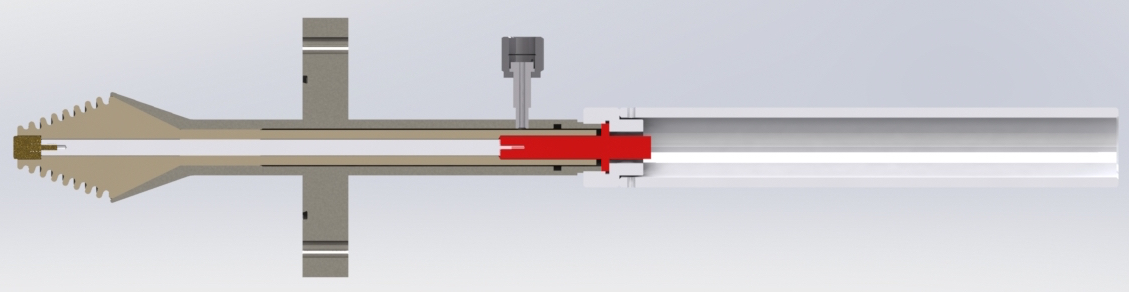
\includegraphics[width=\textwidth]{img2/HVFT_full_image.png}
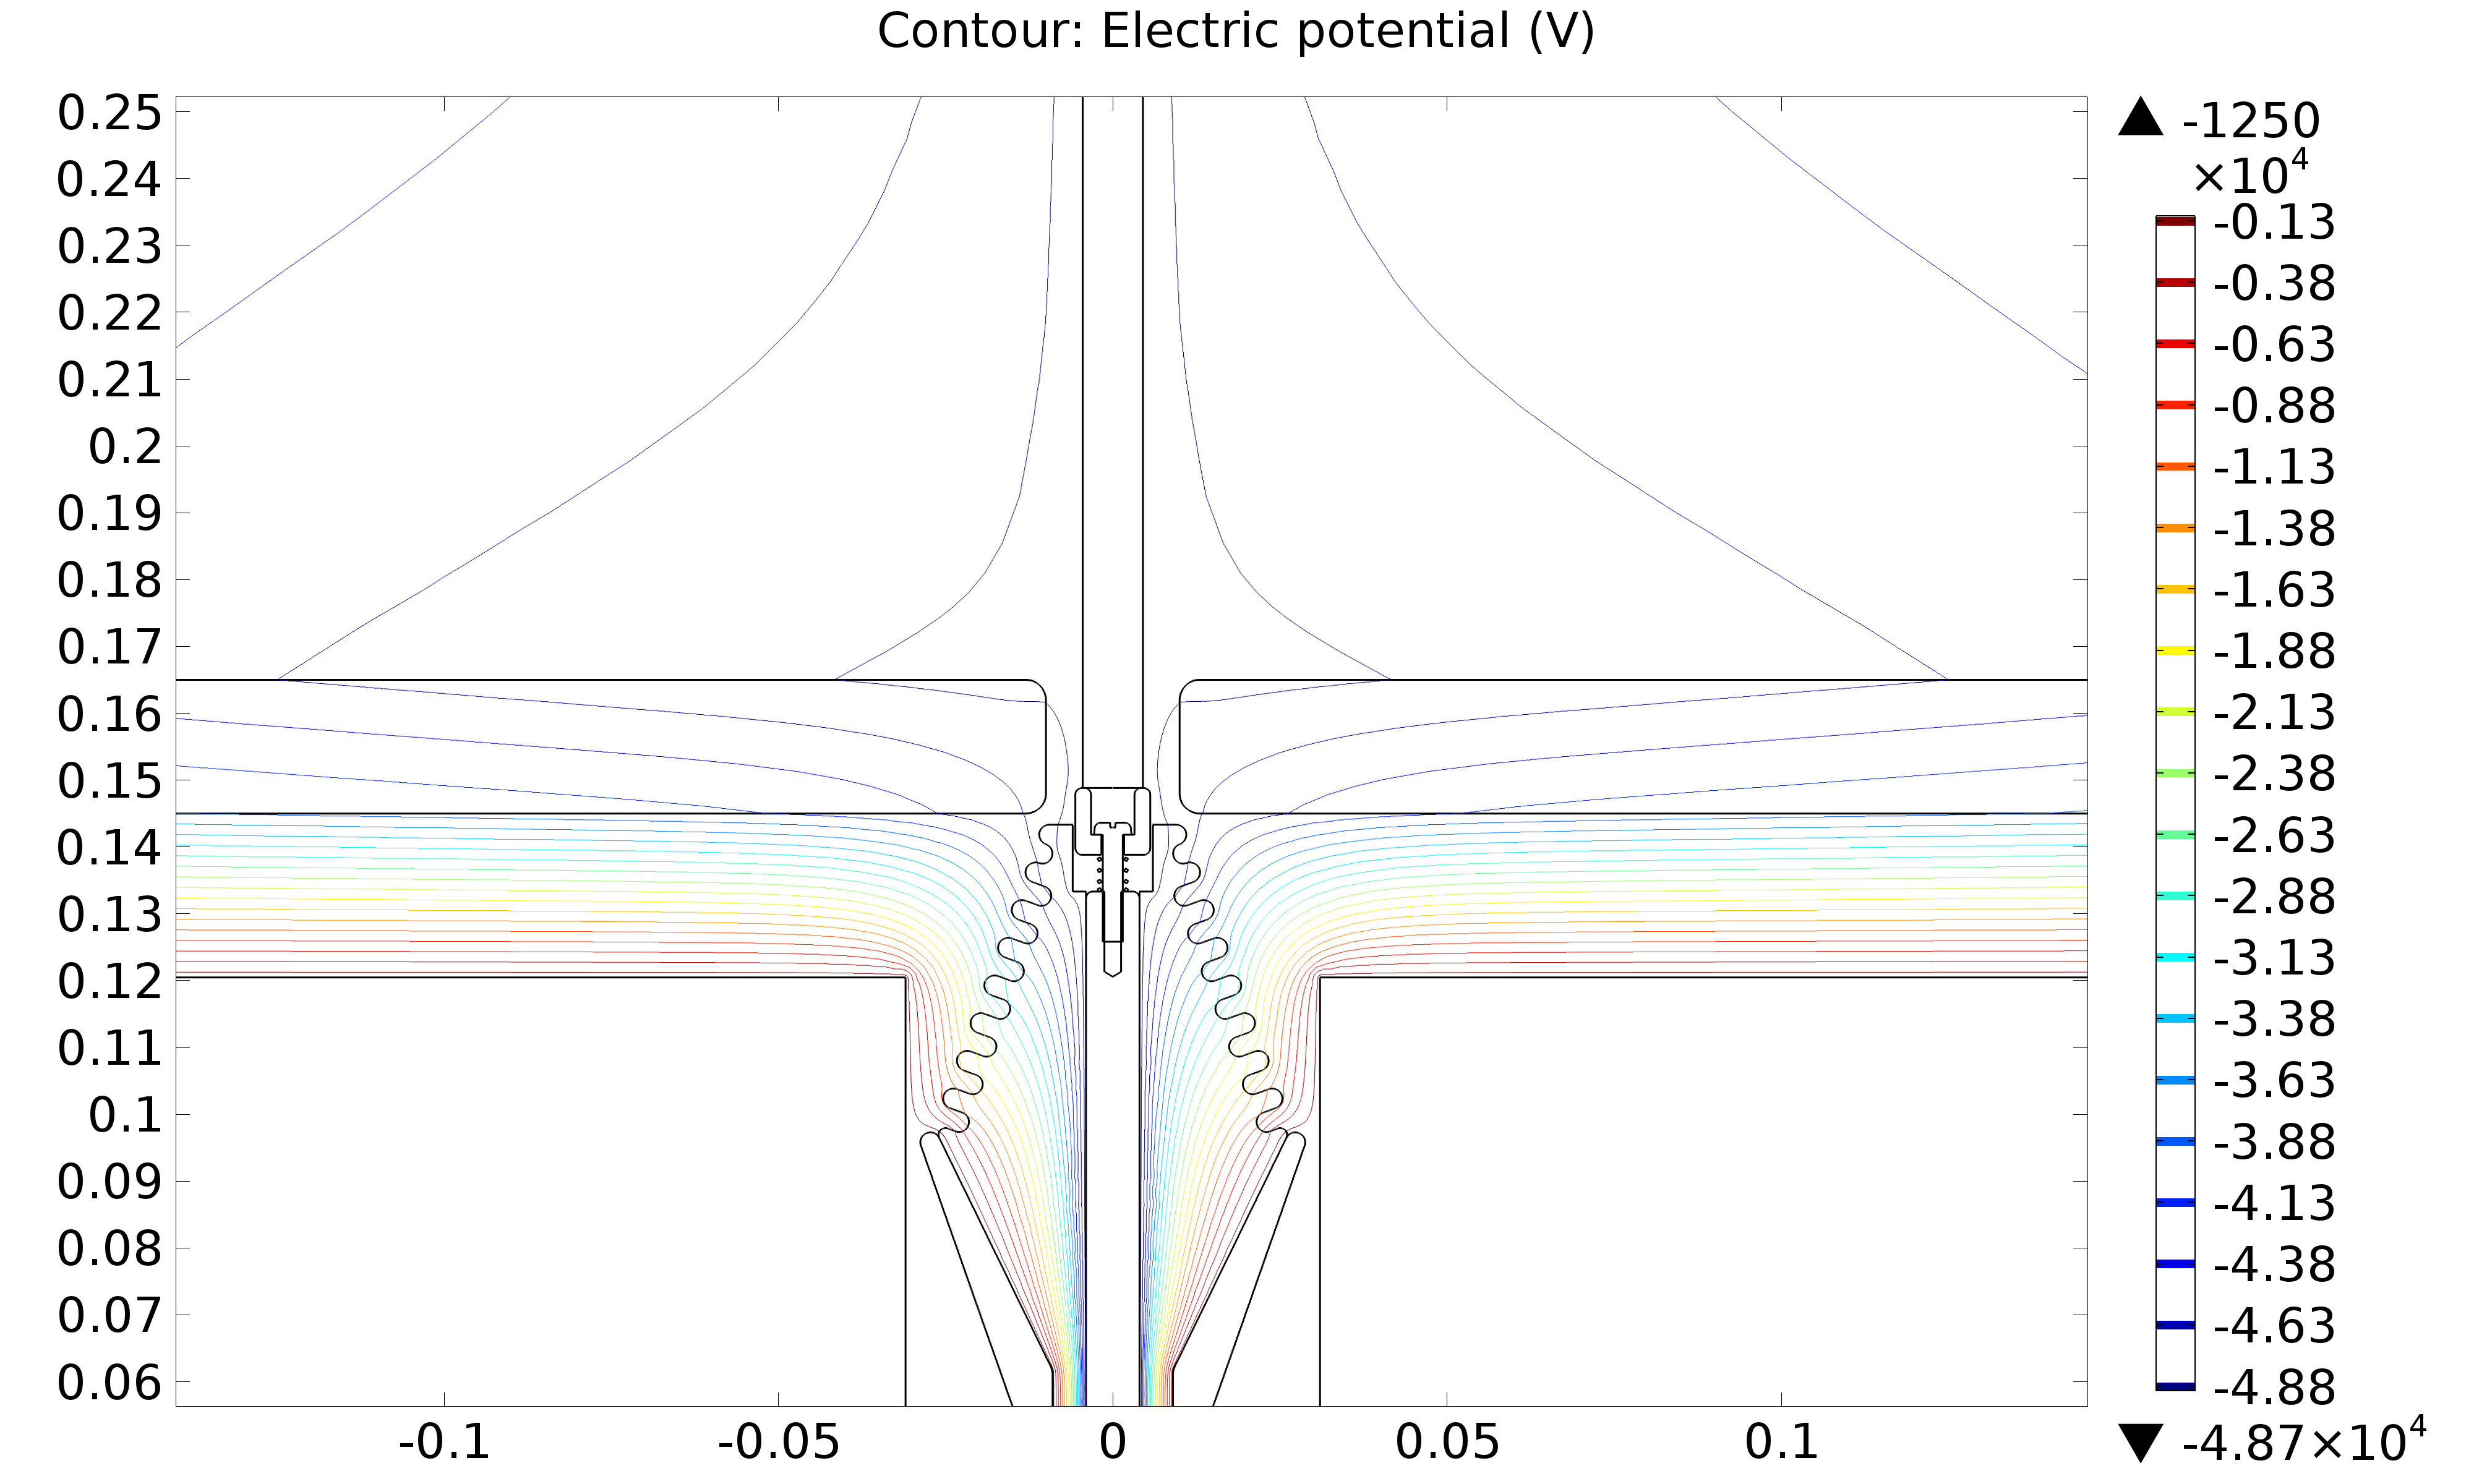
\includegraphics[width=\textwidth]{img2/HVFT_with_drift.png}
\caption{Design (top) and Comsol simulation (bottom) of the NEW HVFT.} \label{fig:hvft1}
\end{figure}


\begin{figure}[hpt!]
\centering
%\includegraphics[width=0.45\textwidth]{FieldCage/img/HVFT_tip_detail.jpg}
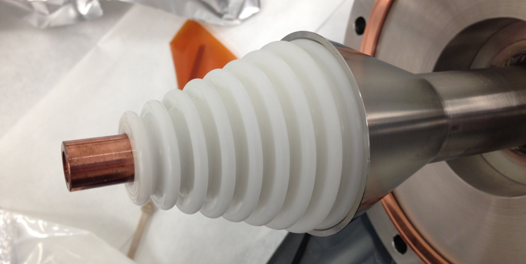
\includegraphics[width=0.75\textwidth]{img2/HVFT2.png}
\caption{A picture of the HVFT.} \label{fig:hvft_tip}
\end{figure}

%\begin{figure}[hpt!]
%\centering
%\caption{Detail of the HVFT tip. The copper conector has been designed  to minimise the electric field in the surface of the tip.} \label{fig:hvft_tip}
%\end{figure}

The most challenging parts of the field cage are the high voltage feedthroughs. These are penetrators which must be capable of holding very high voltages (up to 50 kV for the cathode penetrator and up to 20 kV for the anode) while at the same time being radiopure and gas tight. Figure \ref{fig:hvft1} shows the design of the NEW HVFT. Figure 
\ref{fig:hvft_tip} shows a picture of the cathode HVFT. The initial tests show that the HVFT can hold a voltage in excess of 30 kV with only a few sparks a day. Work is in progress to reduce the number of sparks and increase the maximum voltage. However, 30 kV is sufficient for the initial period of commissioning at 10 bar with a drift field of 15 kV (300 V/cm over 50 cm) and en EL voltage of 15 kV. (E/P $\sim$~3). For NEXT-100 the HVFT needs to withstand 45-55 kV (depending on pressure and EL). Operation with NEW will be essential to improve the performance of the HVFT. 

The cathode grid consist of a stainless steel frame with wires to fix the potential (figure \ref{fig:cath}). It has
been built by the University of Texas A\&M and in currently at the LSC, ready to be installed (first week of May, 2016).

\begin{figure}[hpt!]
\centering
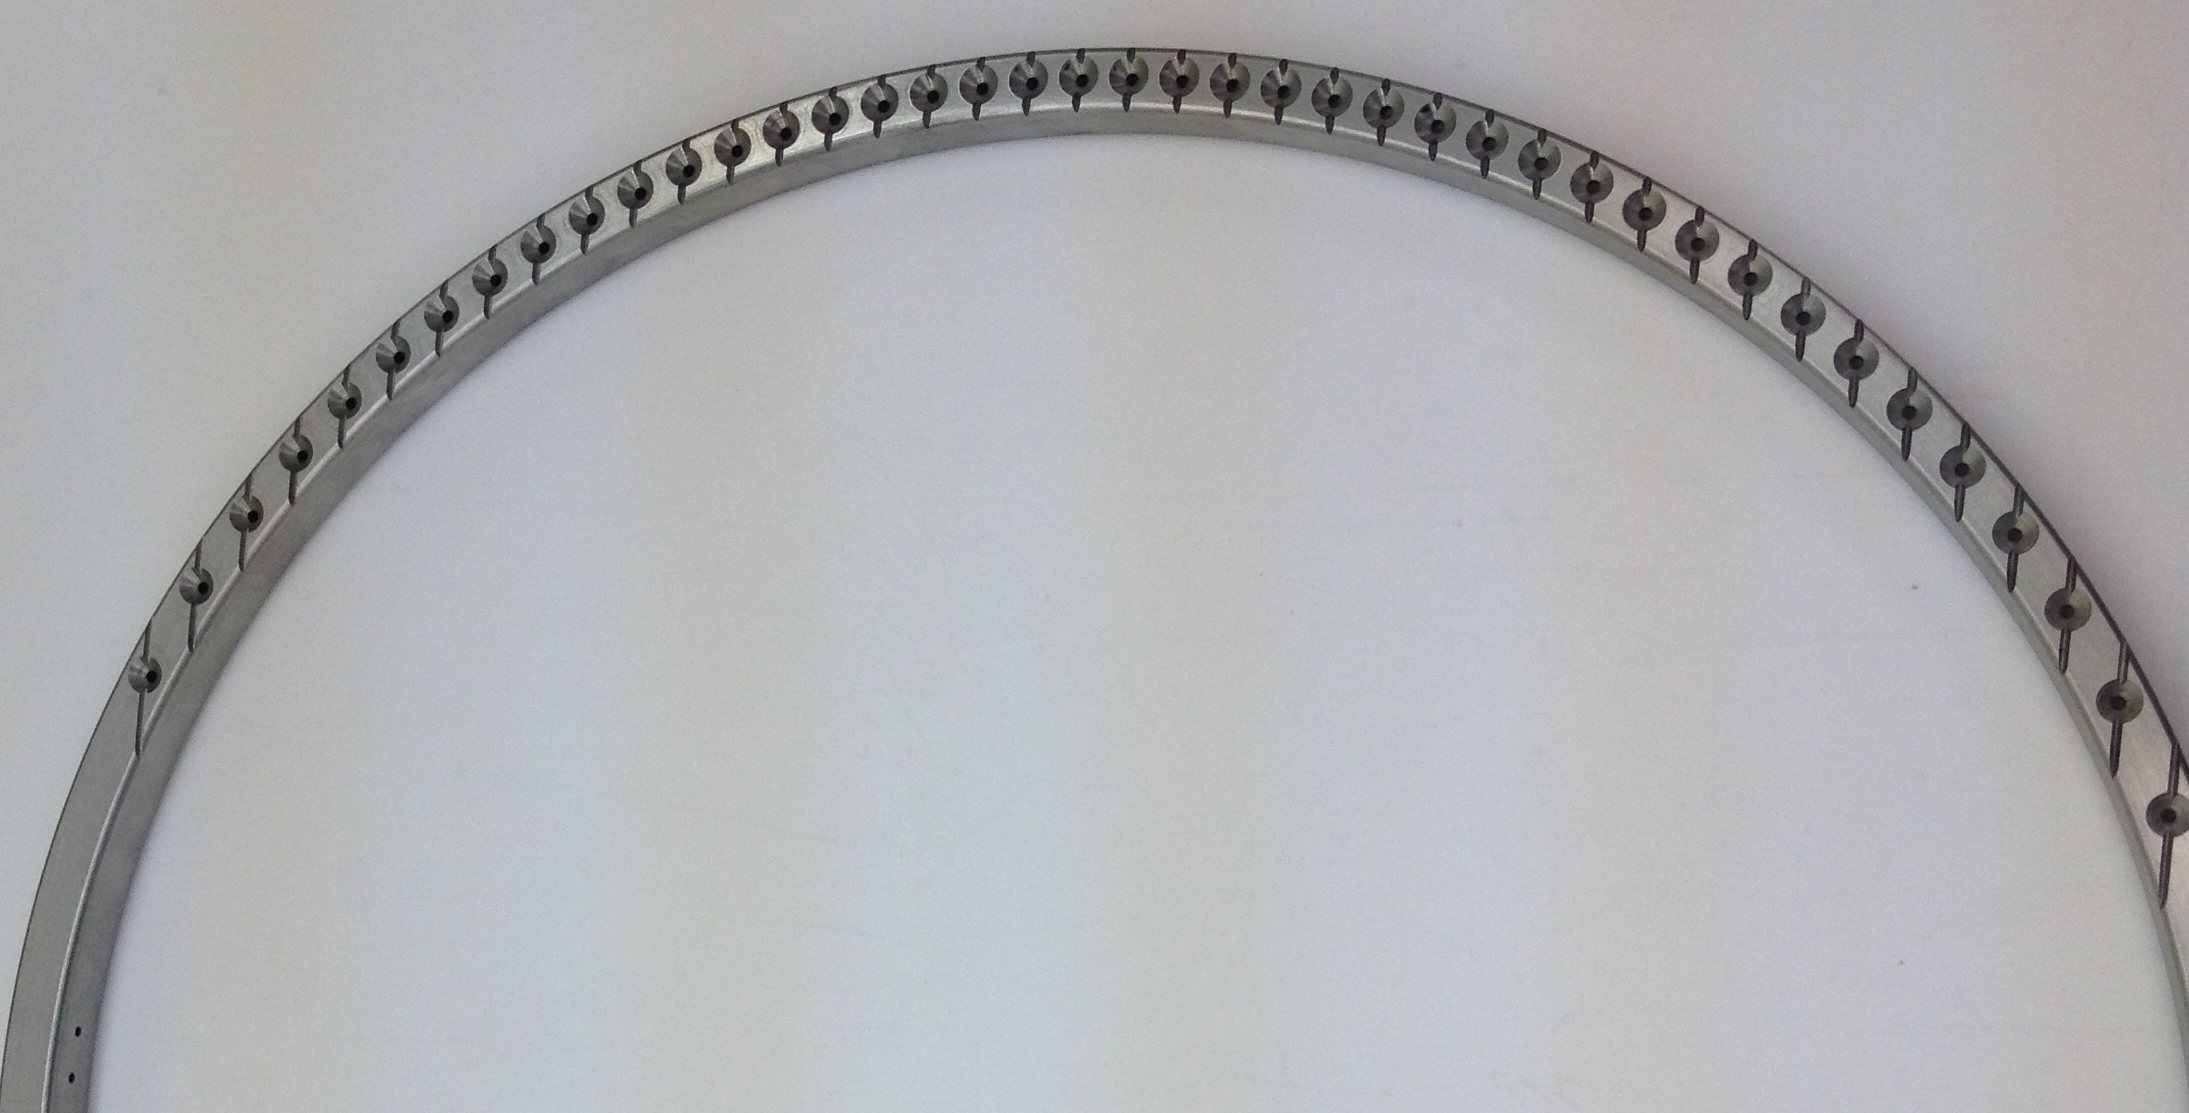
\includegraphics[width=0.45\textwidth]{img2/cathode_1.png}
\includegraphics[width=0.45\textwidth]{img2/cathode_tensioners.png}
\caption{Cathode frame (left) with a detail of the groves for fixing the wires. The bronze tensioners (right) will be used to strength avery wire at the right tension.} \label{fig:cath}
\end{figure}

\begin{figure}[hpt!]
\centering
%\includegraphics[width=0.45\textwidth]{FieldCage/img/mesh_grid_1.jpg}
\includegraphics[width=0.45\textwidth]{img2/SS_grids_1.png}
\includegraphics[width=0.45\textwidth]{img2/Anode_coated.png}
\caption{Top pictures show the  frames used for assembly and tension the gate mesh. Bottom is a picture of the fused silica plate before coating with ITO} \label{fig:el}
\end{figure}

The electroluminescent region (EL) is the amplification region of the detector (figure \ref{fig:el}).  The main parts of the EL are the mesh and the anode. The anode consists in a plate of fused silica coated with ITO in one side and TPB in the other. The fused silica with the layer ITO was produced by Texas A\&M and it arrived at the end of May 2015. It was coated at the LNGS coating facilities and it is ready for installation. The gate mesh is also ready for installation.




%Due to the intensity of the electric field sparks may occur while operating the detector but they will happen inside the detector and so they do not represent a safety issue.

%When installing the detector the fused silica plate needs to be treated very carefull. Only people authorized by the experiment may be allow to do that.






%\section{The NEW project}
% \label{sec.nproj}
%
%\begin{figure}
%\centering
%\includegraphics[width=0.7\paperwidth]{img/NEWProject.pdf}
%\caption{\small The NEW project.}
%\label{fig:NEWProject}
%\end{figure}
%
%The NEW project is organised in terms of sub-projects, called NEW projects or NPR. They are:
%\begin{enumerate}
%\item {\bf Infrastructures}: Construction and commissioning of the mechanical infrastructures (platform, pedestal and lead castle). The project leader is 
%Jose Luis P\'erez (UPV).
%\item {\bf Gas system}: Construction and commissioning of the NEW gas system. The project leader is 
%Igor Liubarsky (IFIC).
%\item {\bf Pressure Vessel}: Construction and commissioning of the NPV, the support table and the opening--closing system. Interfaces with the NFC, NEP and NTP projects. The project leader is 
%Sara C\'arcel (IFIC).
%\item {\bf Field Cage}: Design, construction and commissioning of the NFC, HVFT and EL grids. The project leader is Clement Softka (Texas A\&M). Interfaces with NPV, NEP and NTP.
%\item {\bf Energy plane}: Design, construction and commissioning of the NEP. Interfaces with NFC and NPV. The project leader is 
%Andrew Laing (IFIC).
%\item {\bf Tracking plane}: Design, construction and commissioning of the NTP. Interfaces with NFC and NPV. The project leader is 
%Francesc Monrabal (IFIC).
%\item {\bf FEE}: Design, fabrication and commissioning of the front-end electronics for the PMTs and the SiPMs. Interfaces with NEP and NTP. The project leader is 
%Francisco Toledo (UPV).
%\item {\bf DAQ}: Design, fabrication and commissioning of the data acquisition modules for NEW. Interfaces with FEE. The project leader is 
%Raul Esteve (UPV).
%\item {\bf Slow control}: Design, fabrication and commissioning of the slow control for NEW. Interfaces with all systems that must be controlled. The project leader is 
%Javier Rodr\'iguez (IFIC).
%\item {\bf Online}: Design and commissioning of the online monitoring for NEW. Interfaces with offline, DAQ and Slow Control. The project leader is 
%Toni Mar\'i (UPV).
%\item {\bf Offline}: Design and commissioning of the offline for NEW. Interfaces with online, DAQ and Slow Control. The project leader is 
%Justo Mart\'in-Albo (IFIC).
%\item {\bf Calibration}: Design and commissioning of the calibration systems and procedures for NEW. Interfaces with pressure vessel, field cage and offline. The project leader is 
%Paola Ferrario (IFIC).
%\item {\bf Integration}: Coordinates the integration of the full system at the LSC. The project leader is 
%Teopisti Dafni (UNIZAR).
%\item {\bf Radiopurity}: Coordinates the screening of all the components of NEW and keeps the NEXT background model data base. The project leader is 
%Susana Cebri\'an (UNIZAR).
%\end{enumerate}
%
%
%Figure \ref{fig:NEWProject} shows a summary cronogram of the NEW project. A full resource-load project is being prepared by the technical coordinator (IL) and the spokesperson. The current program allows the construction of NEW and the completion of the needed infrastructures by early 2015. A commissioning period of 6 months is foreseen, followed by at least 12 months of run with enriched xenon. 


